\chapter{Background}
\label{ch:background}

Colliding wind binary (CWB) systems sit at the intersection of many fascinating fields.
Unfortunately this means that a broad swathe of stellar astrophysics must be discussed in order to investigate them in any detail.
In this chapter we will discuss the many underlying subjects of CWB systems.
First, we shall start with massive, early type stars -- how they form, what drives their titanic energy outputs, as well as their inevitable and violent deaths.
Afterwards, we will discuss interstellar dust, the fragile, microscopic grains that act as chemical refineries across the cosmos.
In particular, we will discuss their formation, growth and destruction mechanisms, in order to understand how such an object can arise in such a violent system as a CWB.
We will then move on to discussing colliding wind binary systems, wind parameters and cooling mechanisms.
Finally, we will synthesise what we have discussed by detailing the crux of this project: the dust producing colliding wind binary (WCd) system.
This chapter largely covers the underlying physics of these systems, while the next chapter (Ch. \ref{ch:numsim}) concerns the simulation of these physical phenomena and effects. 

\section{Early-Type Stars}
\label{sec:earlytype}
\label{sec:obtype}

The term Early-type stars is quite possibly the epitome of bad naming conventions in astrophysics.
It's a very old term, coming from the dawn of astrophysics itself, it is quite opaque as to what it means, and is also by definition \textit{completely wrong}.
In fact it is one of the most wrong pieces of terminology I can think of
\footnote{Aside from astrophysicists calling something ``warm'', of course. That can quite literally mean anything from 10 to 1,000,000 Kelvin, depending on who you ask, what they're writing about, or how they're feeling at that particular moment. In fact, I'll probably end up falling into this same trap somewhere in this thesis as well!}.
The first generation of astrophysicists\footnote{As opposed to astronomers or ``natural philosophers''.} found themselves asking very big, very fundamental questions such as ``what even \textit{are} stars?'' and ``what possible mechanism can allow a star to shine for so long?''
Each of these questions was rather pressing for the burgeoning field, and the scientific community was aching for an answer.

Of course, like all pressing questions of the late \nth{19} century, it fell to Lord Kelvin to provide a convincing -- albiet incorrect -- answer.
Kelvin assumed that gravitational collapse was the mechanism for a stars long-term heating, with younger, ``early'' stars shining the brightest.
Not only was the mechanism incorrect, but typically older main sequence stars are more luminous than their younger counterparts of a similar mass!
However, as is the case with astrophysical terminology, the term stuck, to the confusion of many young astrophysicists.
%//FIXME POTENTIAL maybe put this part in with OB stars? allows for more seamless switching from diatribe to the main body
Instead, we now know that stars produce their energy through fusion.
These reactions vary from sub-stellar deuterium and lithium burning, to main sequence p-p \& CNO hydrogen burning processes, and finally to the triple-$\alpha$ and other exotic fusion processes for evolved high-mass stars.
The more massive the star the greater the internal pressure, allowing for more exotic fusion processes.

The bigger a star, the greater the core pressure and temperature.
As all fusion reactions are highly dependent on temperature, stars with only a few dozen solar masses are thousands of times more luminous than our sun -- but only last a fraction of the time \parencite{carrollIntroductionModernAstrophysics2014}.
These stars have luminosities in the range of \SI{1e4}{\solarluminosity} and lifespans on the order of \SI{10}{\mega\year}, less than 0.1\% of the lifespan of our sun.
The adage of a candle burning twice as bright and lasting half as long doesn't quite express the differences between high-mass stars and low-mass stars, it would instead be better to compare a candle and a stick of dynamite.

We define high-mass stars as stars that are sufficiently massive to undergo carbon fusion near the end of their lives.
Defining high-mass as stars that are predominantly driven by the CNO cycle or late-life helium burning can include intermediate mass stars, which form degenerate cores and evolve into white dwarfs.
Many works -- including this one -- define a high-mass, early-type star as having a mass of $>\SI{8}{\solarmass}$.
This includes stars in the O-type and some B-subtype (B0 and B1) classes in the Harvard classification system
\parencite[143]{ward-thompsonIntroductionStarFormation2011}.

% Formation of OB stars, note binary systems!

\subsection{Formation}
\label{sec:starformation}

All stars form from the collapse of giant molecular clouds (GMCs), enormous, cold clouds containing truly staggering amounts of gas.
The largest of these clouds are on the order of a few parsecs across, and contain \SI{1e6}{\solarmass} of potential star-stuff.
These clouds are somewhat stable, and must be perturbed in order to collapse, which is easier said than done, but can be induced by stellar winds from nearby stars, and shock-waves from supernovae
\parencite[Ch.~3]{bodenheimerPrinciplesStarFormation2011}.
As the cloud collapses, energy is radiated through emission line processes, which lowers the radius of thermostatic equilibrium.
As the GMC collapses further it begins to fragment, forming the molecular clumps and cloud cores that will eventually condense into protostars.
As one of these fragments condenses, it forms a proto-stellar core.
This collapse can be described in the form of a series of timescales.
Firstly, the Kelvin-Helmholtz (KH) timescale\footnote{The idea of gravitational contraction as expounded by Lord Kelvin does in fact apply to stars, just not with regards to how their energy is produced.}, $\tau\rms{KH}$, which is the time required for the proto-stellar core to radiate away its kinetic energy:

\begin{equation}
  \label{eq:khtime}
  \tau\rms{KH} \approx \frac{G M_\star^2}{R_\star L_\star},  
\end{equation}

\noindent
where $G$ is the gravitational constant, $M_\star$ is the proto-stellar core mass, $R_\star$ is the radius of the core and $L_\star$ is the core luminosity.
The other timescale is the free-fall timescale, $\tau\rms{ff}$, which is the time taken for a molecular cloud fragment to fully collapse onto the core, given by the equation

\begin{equation}
  \label{eq:fftime}
  \tau\rms{ff} \approx \sqrt{\frac{3\pi}{32 G \rho_\star}} ,
\end{equation}

\noindent
where $\rho_\star$ is the mean density of the collapsing cloud.
The equation of motion for this system is

\begin{equation}
  \frac{d^2r}{dt^2} = - \frac{GM_\star}{r^2} ,
\end{equation}

\noindent
for any point with radius $r$ from the centre in the cloud, assuming spherical symmetry \parencite[96]{ward-thompsonIntroductionStarFormation2011}.

In the case of a massive star, the KH timescale is significantly shorter than the free-fall timescale ($\tau\rms{KH} \ll \tau\rms{ff}$), meaning that the material at the center of the collapsing cloud begins to fuse.
This burgeoning star begins to drive the collapsing material through radiation pressure, blowing this material outwards, causing it to accrete and shock material within the GMC \parencite[Ch.~5]{bodenheimerPrinciplesStarFormation2011}. 

As more massive cores collapse, they are more prone to fragmentation, the angular velocity of the fragments can cause them to begin orbiting one another, eventually forming a binary or multiple star system.
Close binary systems can also form by way of fragmentation in the proto-stellar disk.
Due to this fragmentation it has been observed that roughly 2/3\ts{rds} of all main sequence stars are found to be in a multiple system \parencite[113]{ward-thompsonIntroductionStarFormation2011}, with approximately 20\% of stars in close binary orbits.
However, in the case of massive stars, this value is significantly higher, with $>82\%$ of stars with masses $>\SI{16}{\solarmass}$ being found to be in a close binary system \parencite{chiniSpectroscopicSurveyMultiplicity2012}.
As such, the environment within an OB association is one of many tight knit groups of young stars, which completely disrupt the local area\footnote{This is similar to the environments around student areas, such as Hyde Park and Headingley.}.

\subsection{The p-p \& CNO fusion cycles}

\begin{table}[h]
  \centering
  \begin{tabular}{llll}
    \hline
    Process & Reaction rate & Energy released per nucleon & Significant in \\
    \hline
    p-p & $\epsilon \propto T^{3.5}$ at \SI{5e6}{\kelvin} & \SI{6.54}{\mega\electronvolt} & Low-mass stars \\
    CNO & $\epsilon \propto T^{18}$ at \SI{1e6}{\kelvin} & \SI{6.18}{\mega\electronvolt} & High-mass stars \\
    $3\alpha$ & $\epsilon \propto T^{40}$ at \SI{1e8}{\kelvin}  & \SI{0.61}{\mega\electronvolt} & Post-main-sequence high-mass stars \\
    \hline 
  \end{tabular}
  \caption[Comparison of fusion process reaction rates]{A comparison of reaction rates and released energy for the p-p chain reaction, CNO reaction and triple-alpha reaction. Whilst the $3\alpha$ reaction has a much higher temperature dependence for the reaction, it requires much higher pressures, and produces considerably less energy per nucleon. These factors contribute to the high luminosities and short lifespans of high-mass stars.}
  \label{tab:reactionrates}
\end{table}

\noindent
As we have previously discussed, the KH mechanism is not the driving force behind the generation of energy in a star, instead, this energy is derived through nuclear fusion processes.
We shall briefly discuss the various nuclear fusion processes in order to understand why massive stars are so luminous, as well as how their lives end.
Nuclear fusion in stars was first proposed by \textcite{eddingtonInternalConstitutionStars1920}, though the exact processes continued to be a mystery for nearly 2 decades -- until \textcite{betheEnergyProductionStars1939} discovered the p-p fusion reaction chain that drives approximately 90\% of the energy generation of the sun.
The p-p fusion chain dominates energy generation for stars between $0.08 \,\si{\solarmass} \lesssim \text{M}_\star \lesssim 1.3 \, \si{\solarmass}$, and releases energy by fusing protons into helium in a particularly direct manner: 

\begin{equation}
  \begin{alignedat}{3}
    p + p & \rightarrow \atom{H}{2}{1} + e^+ + \nu_e && ~~ + \SI{1.44}{\mega\electronvolt} \\
    p + \atom{H}{2}{1} & \rightarrow \atom{He}{3}{2} + \gamma && ~~ + \SI{5.49}{\mega\electronvolt} \\ 
    \atom{He}{3}{2} + \atom{He}{3}{2} & \rightarrow \atom{He}{4}{2} + p + p && ~~ + \SI{12.86}{\mega\electronvolt}
  \end{alignedat}
\end{equation}

\noindent
Whilst the reaction is direct and efficient, due to its high energy production per nucleon (Table \ref{tab:reactionrates}), the reaction rate has a poor temperature dependence of $\epsilon \propto T^{3.5}$.
In more massive stars, with core temperatures on the order of $10^8 \, \si{\kelvin}$, the extreme luminosities we observe would simply not occur.
The mechanisms underpinning fusion in intermediate and high-mass stars are much more energetic and temperature dependent.
Above a stellar mass of $1.3 \si{\solarmass}$ pressures and temperatures within a stellar core favour the fusion of hydrogen into helium through the catalytic CNO cycle:

\begin{equation}
  \begin{alignedat}{3}
    \prescript{12}{6}{\text C} + p & \rightarrow \prescript{13}{7}{\text N} && ~~ + \SI{1.95}{\mega\electronvolt} \\ 
    \prescript{13}{7}{\text N} & \rightarrow \prescript{13}{6}{\text C} + e^+ + \nu_e && ~~ + \SI{1.20}{\mega\electronvolt} \\
    \prescript{13}{6}{\text C} + p & \rightarrow \prescript{14}{7}{\text N} + \gamma && ~~ + \SI{7.54}{\mega\electronvolt} \\
    \prescript{14}{7}{\text N} + p & \rightarrow \prescript{15}{8}{\text O} + \gamma && ~~ + \SI{7.35}{\mega\electronvolt} \\
    \prescript{15}{8}{\text O} & \rightarrow \prescript{15}{7}{\text N} + e^+ + \nu_e && ~~ + \SI{1.73}{\mega\electronvolt} \\
    \prescript{15}{7}{\text N} + p & \rightarrow \prescript{12}{6}{\text C} + \prescript{4}{2}{\text {He}} && ~~ + \SI{4.96}{\mega\electronvolt}
  \end{alignedat}
\end{equation}

\noindent
The CNO I cycle -- which was also discovered by \textcite{betheEnergyProductionStars1939} -- has a markedly higher temperature dependence on the reaction rate, $\epsilon \propto 10^{18}$
(\cite[Ch.~10]{wongIntroductoryNuclearPhysics1998}; see Fig. \ref{fig:fusionrates}).
The incredible densities at the cores of high-mass stars therefore result in a reaction rate orders of magnitude higher than the sun.
This results in a convective core surrounded by a radiative envelope, and is the driving force behind the incredible observed luminosities of high-mass stars as they convert hydrogen to helium at a truly astounding rate \parencite[Ch.~5]{salarisEvolutionStarsStellar2005}.

\begin{figure}[h]
  \centering
  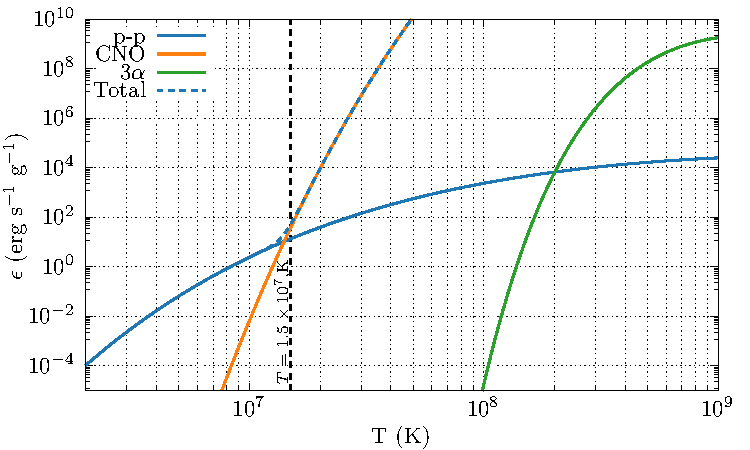
\includegraphics{assets/reaction-rate/reaction-solar.pdf}
  \caption[Reaction rates at the center of the sun]{Reaction rates from p-p, CNO and triple-$\alpha$ fusion processes at the centre of the sun \parencite{harrisThermonuclearReactionRates1983}. At the solar core temperature of \SI{1.5e7}{\kelvin} only 10\% of the energy produced from fusion is through the CNO cycle. At higher internal temperatures the CNO cycle rapidly becomes dominant due to its stronger temperature dependence. The $3\alpha$ process does not occur in the solar core, but becomes the dominant fusion process in high-mass stars leaving the main sequence. Solar abundances and a core density of \SI{150}{\gram\per\centi\metre\cubed} are assumed.}
  \label{fig:fusionrates}
\end{figure}

\subsection{Stellar winds}

% Influence of OB stars on surrounding environment, outsized influence etc.
The luminosities and temperatures of high-mass stars also drive extremely fast stellar winds through radiative line driving.
These winds have on the order of $10^{10}$ times more momentum than winds from stellar-mass stars, and punch holes clean into the interstellar medium (ISM), forming wind-driven bubbles and champagne flows.
These winds can also perturb GMCs, disrupting it and forming more stars nearby.

The study of stellar winds, of course, is quite hard from our vantage point on earth.
Sampling the winds themselves is difficult due to the vast distances involved in sending a probe to collect the rarefied material from our stellar neighbourhood.
% Additionally, the bubble blown from our own suns stellar wind makes collection even more difficult, leaving the heliosphere is no easy feat either, just ask the Voyager probes.
We instead derive the properties of these extrasolar winds from spectrography, with the absorption and emission spectra of the winds betraying their composition.
The velocity of these winds can be determined in much the same manner, through the Doppler shift of these emission lines.
Early observations of stellar winds centred around the star P Cygni, the earliest known example of an evolved Luminous Blue Variable (LBV) star.
The presence of peaks and throughs in the spectra of the star was the cause of some scientific curiosity.
This effect could only be explained by the presence of a shell rapidly expanding away from the star.
The troughs of this spectra corresponded to a blue-shifted adsorption lobe, from radiation passing through this shell, while the emission line itself corresponded to the expanding shell itself \parencite{bealsNatureWolfRayetEmission1929,lamersIntroductionStellarWinds1999}.
Observations of other stars typified this event, it was found that every star had a stellar wind, though the speed and quantity of the ejected material could vary by many orders of magnitude.

% Very basic 
In the simplest terms, we can describe a stellar wind as a spherical outflow from a star.
We can describe this outflow in terms of its mass loss rate, $\mdot$ as well as its terminal velocity, $\vinf$, the maximum velocity a wind can obtain from its driving mechanism.
We can use these to determine a profile of the density of a stellar wind as a function of its distance, $r$, from the star

\begin{equation}
  \rho_w = \frac{\dot{\text{M}}}{4 \pi v^\infty r^2}, \label{eq:smoothwind}
\end{equation}

\noindent
assuming the star is distant enough to behave as a point source.
Whilst this barest description can give us some insight into how a wind behaves, we should discuss the driving mechanisms behind these winds, as well as the more complex models we use to describe them.

\subsubsection{Driving mechanisms}

\begin{table}[h]
  \centering
  % \resizebox{\textwidth}{!}{%
  \begin{tabular}{llll}
  \hline
  \multicolumn{1}{l}{Classification} & \multicolumn{1}{l}{$\mdot$} & \multicolumn{1}{l}{$v_\infty$} & \multicolumn{1}{l}{Mechanism} \\
  \multicolumn{1}{l}{}     & \multicolumn{1}{l}{\si{\solarmass\per\year}}         & \multicolumn{1}{l}{\si{\kilo\metre\per\second}}           & \multicolumn{1}{l}{}          \\ \hline
  Sun            & $10^{-14}$        & 400  & Thermal heating \\
  PMS & $10^{-4}-10^{-7}$ & $200 - 500$ & Rotation \& magnetic fields \\
  Red Giant      & $10^{-7}-10^{-9}$ & 30   & Radiation pressure on dust grains        \\
  OB Star        & $10^{-7}-10^{-8}$ & \num{2500} & Radiation pressure \& line driving      \\
  Wolf-Rayet     & $10^{-5}$         & \num{1500} & Radiation pressure \& line driving       \\ \hline
  \end{tabular}%
  % }
  \caption[Stellar wind comparison]{Comparison of stellar winds emitted from various classification of star.}
  \label{tab:windcomp}
\end{table}

\begin{figure}[h]
  \centering
  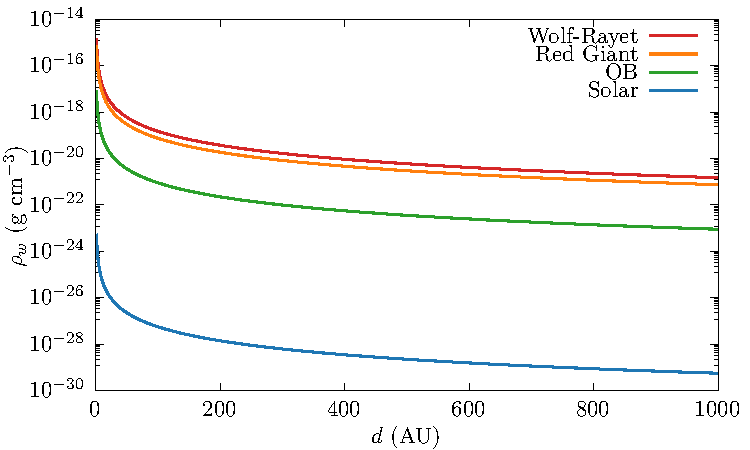
\includegraphics{assets/wind-comparison/wind-comp.pdf}
  \caption[$\rho_w$ comparison of main sequence winds]{Comparison of the densities of various main sequence winds using the parameters specified in table \ref{tab:windcomp}, wind densities are estimated using the smooth wind approximation described in equation \ref{eq:smoothwind}.}
  \label{fig:windrhocomp}
\end{figure}

% Low mass stars
\noindent
Low-mass main sequence stars, compared to other classes of star, have winds that are relatively thin, with a mass loss rate of $10^{-14} \, \si{\solarmass\per\year}$.
Along with their middling velocity of \SI{400}{\kilo\metre\per\second} this results in a wind density many orders of magnitude lower than other types of star (Fig. \ref{fig:windrhocomp}).
The reason for this feeble outflow is the driving mechanism.
The corona in stars with a convective envelope is approximately 3 orders of magnitude hotter than the stars photosphere, this hot corona exerts pressure on gas trapped within it, causing it to be expelled from the star.
This mechanism is thermally driven and does not expel gas from the envelope, only gas dredged up to the corona, explaining this comparative weakness.
In fact, winds from red dwarfs are found to be markedly denser, but the mechanisms behind their winds are less understood.
% Evolved low-mass stars
As low-mass stars evolve and leave the main sequence, they swell into red giants, causing the surface gravity of the star to decrease significantly.
As the star expands and cools, dust condenses and forms in the photosphere.
These dust grains adsorb photons more readily than ions and atoms do through Thompson scattering, and can adsorb a broad range of wavelengths due to their size.
The dust grains are subsequently driven away by radiation pressure, the gas in the wind is coupled to the dust, driving it away in the form of a dense, optically thick, barely supersonic wind
\parencite[Ch.~5]{lamersIntroductionStellarWinds1999}.
The mass loss rates of these stars are extremely high, no lower than $10^{-7} \, \si{\solarmass\per\year}$ and as high as $10^{-5} \, \si{\solarmass\per\year}$ with velocities on the order of $10-100 \, \si{\kilo\metre\per\second}$, making the wind extremely dense.

% High mass stars

By the 1970s the winds of early-type stars had been typified, finding mass loss rates between $10^{-8}$ to $10^{-5} \, \si{\solarmass\per\year}$ and wind velocities of \num{600} to \SI{3500}{\kilo\metre\per\second}.
It was also found that the mass loss rate of these stars was almost proportional to the luminosity ($\mdot_\star \propto L_\star^{1.1}$; \cite{cassinelliStellarWinds1979}).
This strongly suggested that the driving mechanism of these winds was based on radiation pressure, though thompson scattering would not be a sufficiently efficient process to drive winds of this magnitude.
Furthermore, coronal heating and dust driving mechanisms were not possible, due to a lack of a convective envelope and lack of dust build up respectively.

\subsubsection{Line-driven wind theory}
\label{sec:cak}

\begin{figure}[h]
  \centering
  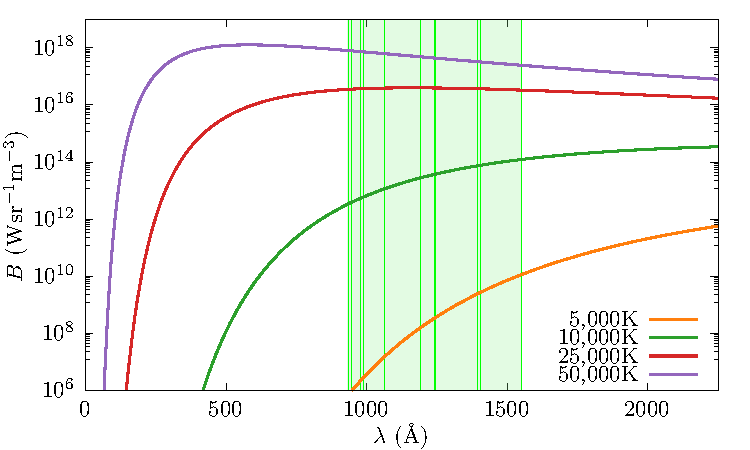
\includegraphics{assets/plancks-law/plancks-law.pdf}
  \caption[Planck's law radiance comparison with resonance lines]{Spectral radiance against wavelength for black body objects at various effective temperatures, $T_{\text{eff}}$, a series of wavelengths corresponding with important resonance lines in Table 1 of \textcite{lucy_mass_1970} have been included. As temperature increases the spectral radiance at resonance line wavelengths dramatically increases, with a minimum of 6 orders of magnitude difference between the effective temperatures of a solar equivalent main sequence star and an O-type main sequence or Wolf-Rayet star.}
  \label{fig:planck-comp}
\end{figure}

% Line driven wind theory 
Line-driven winds present an alternative driving mechanism for massive stars.
A photon with an energy equal to the excitation energy of an emission line of an ion in the wind is adsorbed, exciting the ion.
This ion then de-excites over a timescale of $10^{-8} \, \si{\second}$, emitting a photon at a random angle relative to the radial direction relative to the star, $\alpha$.
This emission of a photon produces a recoil force on the ion, resulting in a change in the radial velocity, $\Delta v\rms{r}$, such that:

\begin{equation}
  \Delta v\rms{r} = v\rms{r}'' + v\rms{r}' - v\rms{r} = \frac{h\nu_0}{mc} \left(1-\cos \alpha \right),
\end{equation}

\noindent
where $v\rms{r}'$ is the ions radial velocity after the photon adsorption, $v\rms{r}''$ is the ions radial velocity after photon emission and $\nu_0$ is the frequency of the resonating photon.
Compared to conventional Thompson scattering, resonance lines are six orders of magnitude more opaque, making it a much more efficient process
\parencite[Ch.~8]{lamersIntroductionStellarWinds1999}.
This driving force occurs in winds enriched with elements with a large number of resonant lines, where heavier ion species from C, N, O and Fe group elements adsorb the photons.
Lighter elements such as H and He are carried along via Coulomb forces, coupled to the heavier elements so long as the medium is sufficiently dense.

But why is this effect not observed in lower mass stars?
Resonance lines in heavier elements have comparatively high energy transitions, requiring ionising UV photons to excite them. 
For instance, the C III resonance line has an energy of \SI{12.69}{\electronvolt}, so a photon requires a wavelength of \SI{977}{\angstrom} in order to be adsorbed (Fig. {\ref{fig:planck-comp}}).
Additionally, photons would only be adsorbed over a narrow range of frequencies.
This inhibits efficient momentum transfer from UV photons without Doppler shift.
As the outflow from the star has a distribution of radial velocities this results in a greater chance of resonance line adsorption if Doppler shift is considered.
If we were to observe the outflow of a massive wind we observe a relatively low velocity component of the wind close to the star once the wind reaches a certain critical velocity.
At a certain point we would observe a significant and rapid increase in the velocity of the wind, as the influence on adsorption due to Doppler shift results in the wind becoming much more opaque to UV photons.
Eventually we would observe the wind reaching a terminal velocity, due to a decrease in photon flux from the inverse square law and the outflow becoming more diffuse as it spreads away from the star \parencite[Ch.~10]{macielHydrodynamicsStellarWinds2014}.
This can be seen in Fig. \ref{fig:cak-vel}, where the velocity increases sharply at a distance $(R/R_\star) - 1 > 10^{-3}$ as the wind begins to rapidly accelerate away from the star as opacity increases -- with a corresponding decrease in wind density.

\begin{figure}[h]
  \centering
  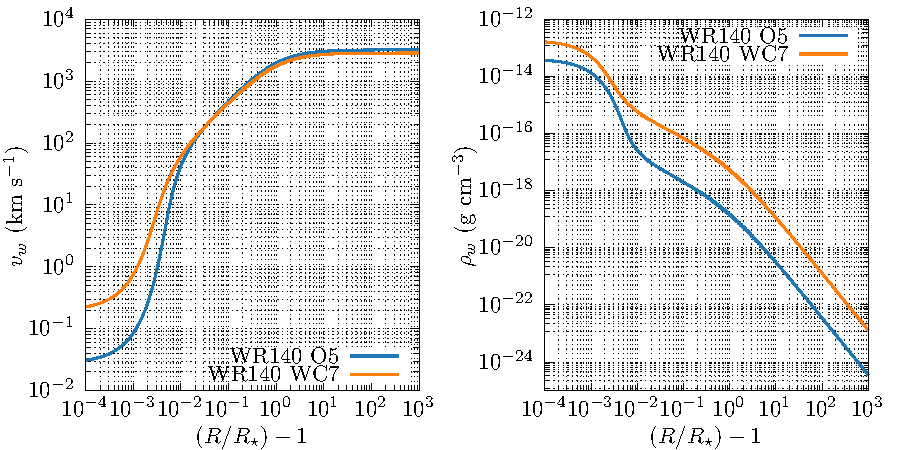
\includegraphics[]{assets/cak/vel.pdf}
  \caption[Radiative line driving velocity and density profile]{Velocity and density profiles of the WR and OB stars in the WR140 system. Acceleration is gradual until $(R/R_\star) - 1 > 10^{-3}$, where wind opacity drastically increases due to Doppler shift. The model uses the Castor, Abbott and Klein formalism, with the CAK parameters of the stars estimated to be $k = 0.37$, $\alpha = 0.60$ for the O4-5 star and $k = 0.48$, $\alpha = 0.57$ for the WC7 star.}
  \label{fig:cak-vel}
\end{figure}

Theories of radiation pressure being the main driving force for massive stars was first considered by astronomers in the early \nth{20} century, and was first proposed by \textcite{sahaRadiationPressureQuantumTheory1919}.
Later, \textcite{milnePossibilityEmissionHighspeed1926} predicted that after an initial acceleration phase from an ions emission lines, Doppler shift would be sufficient for continuum photons frequencies to match the resonant lines -- causing a much greater impulsive force.
Early calculations of the force on stellar winds due to resonance lines by \textcite{lucy_mass_1970} found initial estimates for the mass loss rate based on a series of resonance line in the C, N, Si and S species of ions.
However these were found to underestimate the mass loss by approximately two orders of magnitude.
This is in part due to the models simplicity, due to limitations in both computing power and available data, as the force due to interaction of resonance lines with continuum photons were considered.
The first major breakthrough was with more complex models demonstrated by Castor, Abbott and Klein (\citeyear{castor_radiation-driven_1975}; abbreviated to CAK).
The CAK model computed line forces from all emission lines in the C III ion, after estimating the line force from other ions by scaling the results of this calculation an estimate of mass loss rates for hot stars was calculated to within a factor of 3 of observational results.
A much more complex emission line model developed by \textcite{1982ApJ...259..282A} involved the calculation of the force from a startling \num{250000} lines, however, this was found to be less accurate than the original CAK model!
As researchers went back to the drawing board, improvements were made to the approximations and assumptions made by the CAK model, such as the finite disk correction factor
\parencite{friend_theory_1986,pauldrachRadiationdrivenWindsHot1986}.

\subsection{Evolved early-type stars}
\label{sec:evolvedstars}
% Evolution and fate of massive stars, evolution, depletion of hydrogen products, then onto helium burning
Unfortunately for the most massive stars, pesky limitations such as the conservation of energy severely curtail their lifespans.
Despite being anywhere from 3 to 6 orders of magnitude brighter, the most massive stars typically have between 1 and 2 orders of magnitude more mass to fuse.
% As such, they simply cannot compete with the ten billion year lifespan of our sun, or red dwarfs, which can have lifespans in the \emph{trillions} of years!
% Luminosity lifetime relation
% In order to approximate the main sequence lifespan of a massive, early-type star we must make some assumptions.
We can assume the main sequence lifespan of a star is determined by the amount of available hydrogen in the star as well as the fusion rate of the star.
We can therefore estimate this lifespan, $\tau_\star$, through the equation

\begin{equation}
  \tau_\star \approx \frac{\mass_\star}{\lumin_\star} ,
\end{equation}

\noindent
where $\mass_\star$ is the mass of the star and $\lumin_\star$ is the luminosity of the star.
Through observation a mass-luminosity relation was derived \parencite[139]{salarisEvolutionStarsStellar2005}, such that:

\begin{equation}
  \frac{\lumin_\star}{\lumin\sol} \propto
  \begin{cases}
    \mass_\star / \mass\sol^{2.6} , & \text{if } \SI{0.2}{\solarmass} \lesssim \mass_\star \lesssim \SI{0.5}{\solarmass} \\
    \mass_\star / \mass\sol^{4.5} , & \text{if } \SI{0.5}{\solarmass} \lesssim \mass_\star \lesssim \SI{2}{\solarmass} \\
    \mass_\star / \mass\sol^{3.6} , & \text{if } \SI{2}{\solarmass} \lesssim \mass_\star \lesssim \SI{20}{\solarmass} .
  \end{cases}
\end{equation}

\noindent
We can then make the following estimate for the main sequence lifespan of an early-type star:

\begin{equation}
  \label{eq:mass-lifespan}
  \tau_\star \approx \tau\sol \left(\frac{\mass_\star}{\mass\sol}\right)^{-2.5}.
\end{equation}

\noindent
Whilst this is a fairly simplistic reduction of the stellar mass loss rate, more advanced models such as the Modules for Experiments in Stellar Astrophysics (MESA) project show that this estimate is somewhat accurate.
As we can see in Fig. \ref{fig:mist-lifespan}, this estimate is somewhat accurate over near-solar mass and some lower mass early-type stars.
Assuming a solar lifespan of $\tau\sol = \SI{10}{\giga\year}$ we find through Eq. \ref{eq:mass-lifespan} that a typical O-type star with a mass of \SI{10}{\solarmass} has a main-sequence lifetime of $\sim \SI{30}{\mega\year}$.
It takes the sun approximately \SI{230}{\mega\year} to orbit the galaxy, making the suns ``age'' approximately 19 galactic ``years'' old. Continuing with this analogy, we find that even the least luminous early-type star does not make it to its first birthday!

\begin{figure}[ht]
  \centering
  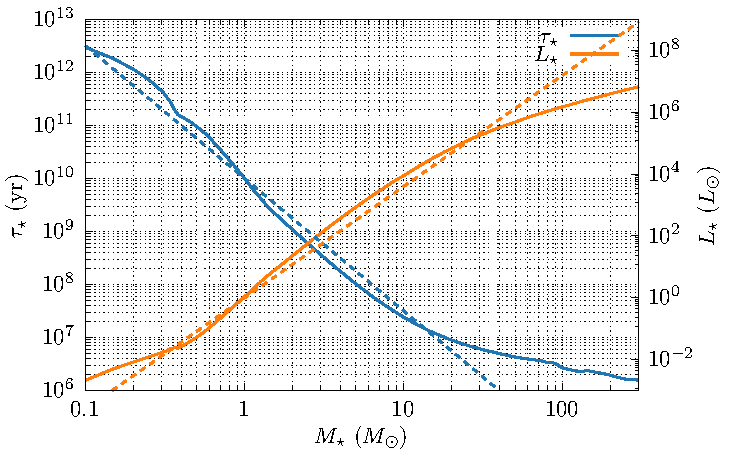
\includegraphics{assets/lifespan/lifespan.pdf}
  \caption[Luminosity and lifetime as a function of stellar mass]{A comparison of luminosity and lifetime as a function of initial stellar mass. An estimate of the stellar lifetime of $\tau_\star \approx \tau\sol (\mass_\star/\mass\sol)^{-2.5}$ and an estimate for luminosity of $L_\star \approx L \sol (\mass_\star/\mass\sol)^{3.6}$ are overlaid with a dashed line. We can see that these estimates are suitable for stars $\lesssim 20 \, \mass\sol$. Lifetime and luminosity data was derived from the MESA Isochrones and Stellar Tracks (MIST) project \parencite{choiMesaIsochronesStellar2016,dotterMESAIsochronesStellar2016,paxtonModulesExperimentsStellar2011}.}
  \label{fig:mist-lifespan}
\end{figure}

% Running out of fuel, schonberg
Eventually, the hydrogen in a massive stars core is completely exhausted, leaving an inert helium core with a hydrogen envelope surrounding it.
Near the edge of the depleted core, the temperature is still sufficient for hydrogen to burn, with energy production in the star transitioning to a shell-burning process.
\textcite{schonbergEvolutionMainSequenceStars1942} determined that as the star transitions from core to shell H-burning the temperature gradient in core and envelope is radiative, with an isothermal stratification.
Due to this, there is a limiting factor on the stable core size of a star.
Above this \emph{Sch{\"o}nberg-Chandrasekhar} limit ($q\rms{SC}$) the core contracts on the KH timescale (Eq. \ref{eq:khtime}), with the limit determined by the ratio of the mean molecular mass, $\mu$, of the envelope and the core, such that:

\begin{equation}
  q\rms{SC} \equiv \left(\frac{\mass\rms{core}}{\mass\rms{tot}}\right)\rms{SC} = 0.37 \left(\frac{\mu\rms{env}}{\mu\rms{core}}\right)^2 .
\end{equation}

\noindent
For a star of solar composition we find $q\rms{SC} \sim 0.08$
\parencite[Ch.~5]{salarisEvolutionStarsStellar2005}.
For low-mass stars, this collapse timescale is extremely slow.
Instead the star expands into an asymptotic giant branch (AGB) star, continuing shell burning until the material is exhausted
\parencite{beechSchoenbergChandrasekharLimitPolytropic1988}.
This leaves behind a degenerate helium core in the form of a white dwarf, which continues to contract and emit radiation through KH processes\footnote{Finally! Kelvin was right!}.

For massive stars the ratio of core mass to total mass is significantly higher, exceeding the Sch{\"o}nberg-Chandrasekhar limit.
The outer envelope is driven away through radiation processes as the calculus of hydrostatic equilibrium shifts from contraction to expansion.
The star then balloons into a red supergiant (RSG) star or an LBV star.
Inside this giant star the core continues to collapse, compressing and heating further, eventually reaching temperatures sufficient for the commencement of helium burning through the Triple-$\alpha$ (3$\alpha$) process:

\begin{equation}
  \begin{alignedat}{3}
    \atom{He}{4}{2} + \atom{He}{4}{2} & \rightleftarrows \atom{Be}{8}{4} && ~~ - \SI{0.09}{\mega\electronvolt} \\
    \atom{Be}{8}{4} + \atom{He}{4}{2} & \rightarrow \atom{C}{12}{6} + 2\gamma && ~~ + \SI{7.37}{\mega\electronvolt} 
  \end{alignedat}
\end{equation}

\noindent
% Which can also produce a small amount of oxygen with an additional $\atom{C}{12}{6} + \atom{He}{4}{2}$ interaction.
The endothermic component of the 3$\alpha$ process, as well as the short reaction time prevents it from occurring in any reasonable quantity until core temperatures are in the order of hundreds of millions of Kelvin
\parencite[Pt.~6]{kippenhahnStellarStructureEvolution2012}.
The reaction rate of the 3$\alpha$ process is proportional to $T^{40}$, which can result in staggering amounts of energy production.
This process is far less energy efficient than hydrogen burning processes, and releases an order of magnitude less energy per nucleon (Table \ref{tab:reactionrates}), hence, the helium burning process can be as short as \SI{500000}{\year}.
At this point the fate of the star is sealed, it hurtles off of the main sequence like a 1966 Ford Thunderbird from the edge of the Grand Canyon\footnote{See \emph{Thelma and Louise} (1991) dir. Ridley Scott.}.
Because of this helium burning, the most massive of early-type stars transition into a Wolf-Rayet (WR) star -- one of the cruces of this thesis.

\subsubsection{Wolf-Rayet stars}
\label{sec:wrtype}

\begin{figure}[ht]
  \centering
  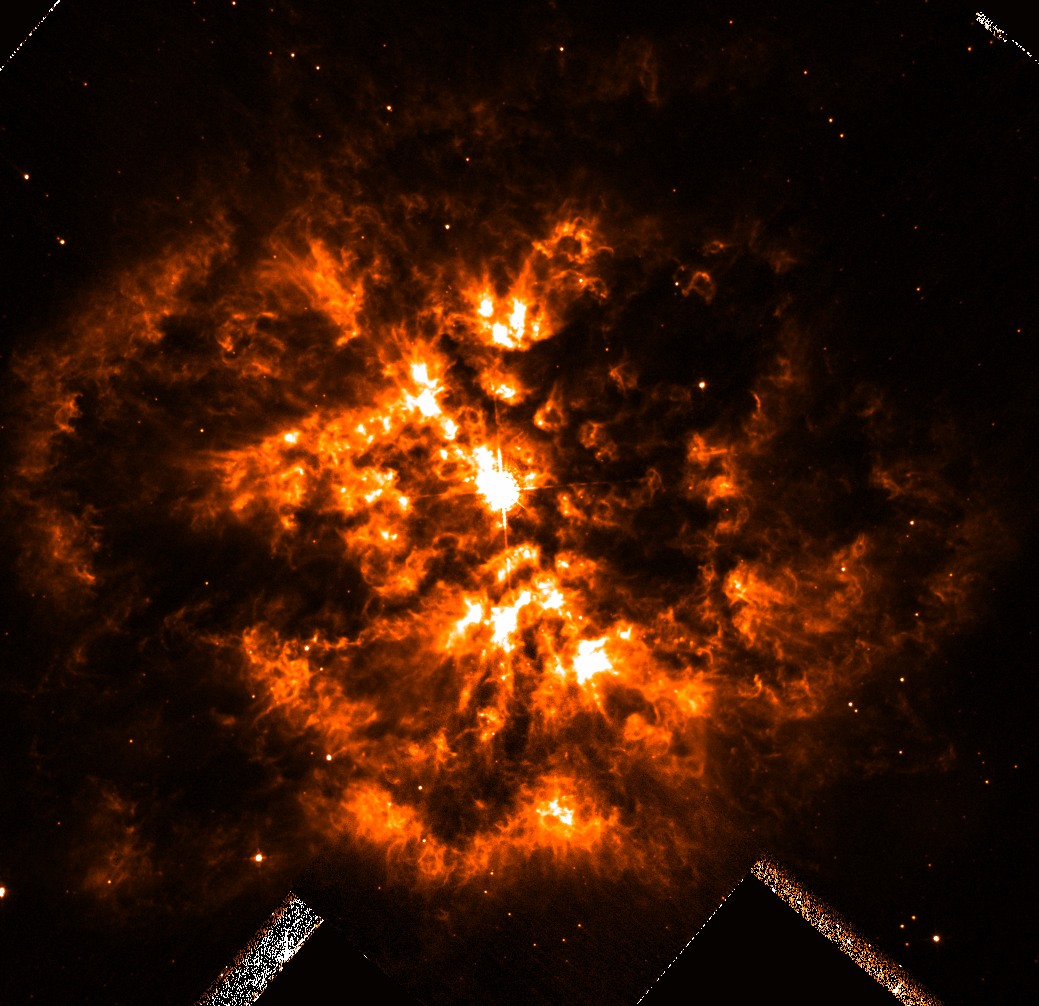
\includegraphics[width=4in]{assets/WR124.png}
  \caption[\textit{M1-67 nebula around WR124 \parencite{2010ApJ...724L..90M}}]{Reduced Hubble WFPC2 data of the WN star WR124, its extreme mass loss is currently producing the ejecta nebula M1-67 \parencite{2010ApJ...724L..90M}.}
  \label{fig:wr124}
\end{figure}

% History of observation

\noindent
In the late 19\ts{th} century, astronomers Charles Wolf and Georges Rayet noted a curious series of stars with exceptionally broad emission lines.
Considering that stars previously had only been observed with narrow adsorption lines, this was a particular scientific curiosity
\parencite{crowther_physical_2007}.
While the mechanism behind energy production in stars was not understood, the scientific community did understand that these winds were \emph{staggeringly} hot.
After the initial theories of stellar fusion reactions were developed by \textcite{betheEnergyProductionStars1939}, however, the picture came into sharper focus.
\textcite{gamowWCWNStars1943} proposed that these stars contained material produced in the central fusion reaction, which implied that the outer layers of the star had been completely stripped off.
This was found to be the case, though categorical confirmation of this did not occur for several more decades.
The thickness of these emission lines was easier to establish -- these ions were moving \emph{fast}.
As such, it was safe to assume that the emission lines were not coming from the stars themselves, but from the winds!

% Evolution, include crowther table here

\begin{figure}[ht]
  \centering
  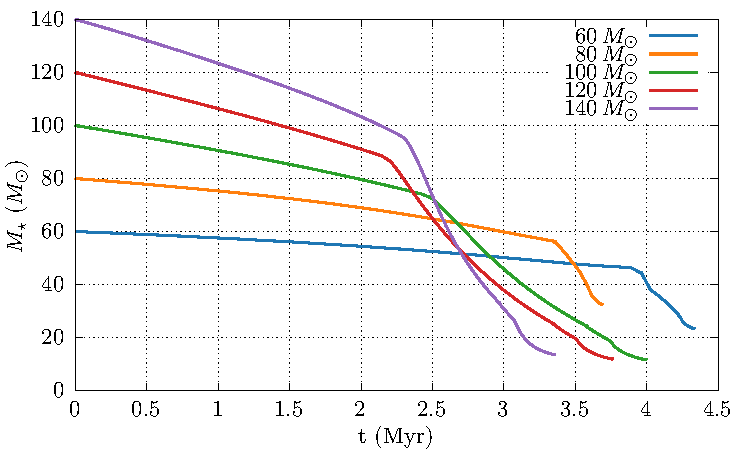
\includegraphics{assets/massloss/massloss.pdf}
  \caption[Examples of mass loss over the lifetime of a high-mass star]{Examples of mass loss over the lifetime of a high-mass star. High mass stars clearly undergo significant mass loss as they transition into evolved LBV and WR stars. In all cases we see a reduction in mass loss rate during the terminal WR stage of their lives, and that the stars have shed well over half of their initial mass before entering their WR phase. Stellar evolution data was derived from the MIST project \parencite{choiMesaIsochronesStellar2016,dotterMESAIsochronesStellar2016,paxtonModulesExperimentsStellar2011}.}
  \label{fig:mist-massloss}
\end{figure}

Wolf-Rayet (WR) stars are produced when the largest early-type stars lose significant mass in the LBV stage (Fig. \ref{fig:wr124} \& \ref{fig:mist-massloss}), while the internal core has the sufficient pressure and temperature required for helium burning.
This drives the remnants of the outer envelope away, exposing more and more of the innards of the star, the inner envelope and core, which are still burning hydrogen and helium
\parencite[Ch.~5]{contiLuminousHotStars2012}.
% Mass loss rates, wind velocities
Whilst in the LBV phase mass loss rates can be higher, these are short but intense bursts of mass loss, rather than a continuous wind \parencite[Ch.~4]{vinkVeryMassiveStars2015}.
WR stars, in comarison, drive significant, continuous mass loss of the order of $10^{-5} \, \si{\solarmass\per\year}$, with wind velocities on the order of $10^3 \, \si{\kilo\metre\per\second}$. 
% Wind temperatures adn composition, emission lines?
The naked core has an extremely high surface temperature, between \SI{30000}{\kelvin} to \SI{100000}{\kelvin}, multiply ionising the outflowing hydrogen-deprived wind
\parencite{crowther_physical_2007}.
The temperature of this heat source also produces significant emissions in the far-UV, which drives the exceptional mass loss through radiative line driving.
As the Wolf-Rayet evolves, layers of this burning region are stripped away from the surface of the star, contributing to the stellar wind.
Because of this, the outflow becomes more hydrogen-depleted as the star ages, becoming more enriched with fusion by-products, helium, carbon, nitrogen and oxygen.

% Subtypes
Wolf-Rayets can also be subdivided into three distinct categories based on their prominent emission lines:

\begin{itemize}
  \item WN: WR stars with a strong nitrogen emission line sequence, some helium lines.
  \item WC: WR stars with a strong carbon emission line sequence, some oxygen lines.
  \item WO: WR stars with a strong oxygen emission line sequence, some carbon lines.
\end{itemize}

\noindent
Further subdivision can be done by measuring the brightness of these emission lines, for example, the WC4 subtype are the dimmest WC stars, with ascending values being brighter.
Previously this measurement was more qualitative, and based on the relative ratio of line strengths, however more quantitative methodologies of categorising these stars have emerged
\parencite{crowtherQuantitativeClassificationWC1998}.
% Conti scenario
\textcite{contiRelationshipWRStars1975} first proposed that massive stars would lose their outer envelopes while undergoing core helium burning.
Initially the outermost hydrogen layer is ejected from the star, which is observed as a WN phase WR.
As the star continues to evolve and the remaining envelope becomes helium depleted, we observe emission from the exposed core and innermost, carbon and oxygen enriched shell
\parencite{neugentWolfRayetContent2019,oswaltPlanetsStarsStellar2013}.
The ``Conti scenario'' that they described forms the basis for stellar evolution models from main sequence O-type stars to Wolf-Rayet stars.
Further work has refined this evolutionary chain.
Successive and intermediate stages occur depending on the initial mass of the O-type star, $\mass\rms{O}$.
\textcite{crowther_physical_2007} details this series of evolution modes for O-type stars evolving into WR stars:

\begin{equation}
  \label{eq:wrevolution}
  \text{O} \rightarrow
  \begin{cases}
    \text{LBV/RSG} \rightarrow \text{WN} \rightarrow \text{SN Ib} & \text{ for } \SI{25}{\solarmass} < \mass\rms{O} < \SI{40}{\solarmass} \\
    \text{LBV} \rightarrow \text{WN} \rightarrow \text{WC} \rightarrow \text{SN Ic} & \text{ for } \SI{40}{\solarmass} < \mass\rms{O} < \SI{75}{\solarmass} \\ 
    \text{WN(H-rich)} \rightarrow LBV \rightarrow \text{WN} \rightarrow \text{WC} \rightarrow \text{SN Ic} & \text{ for } \mass\rms{O} > \SI{75}{\solarmass} .
  \end{cases}
\end{equation}

% Discussion of 
\noindent
This can also be seen in evolutionary tracks, such as those in Fig. \ref{fig:mist-zams}.
WC stars form from the most massive of O-type stars, and are the only observed dust-producing WR stars.
% WC stars, in particular, why important
The hydrogen in a WC stars envelope has been completely depleted, instead, the stellar wind is enriched with other elements such as helium, carbon and oxygen.
The presence of large quantities of carbon in the outflow is of particular interest, as interstellar dust can condense and form.
Whilst low quantities of interstellar dust have been observed in the vicinity of single WC stars, this is typically in very low amounts.
Certain binary systems can produce quantities of dust that can significantly impact their local environment, however.
Within a binary system, it is typically paired with another massive star, such as an O-type or B-type.
The RSG/LBV phase strips off the bulk of the stars outer envelope, resulting in a WR star that is significantly smaller and lighter than its partner.
Despite this, the strong winds produced by the WR star completely dominate the winds of its larger compatriot.
If these stars are sufficiently close these winds interact, driving extremely powerful shocks, extreme x-ray fluxes and the aforementioned dust formation.
These binaries will be discussed in much more detail -- of course -- as they are the central objects of this thesis (Section \ref{sec:cwb}).

\begin{figure}[ht]
  \centering
  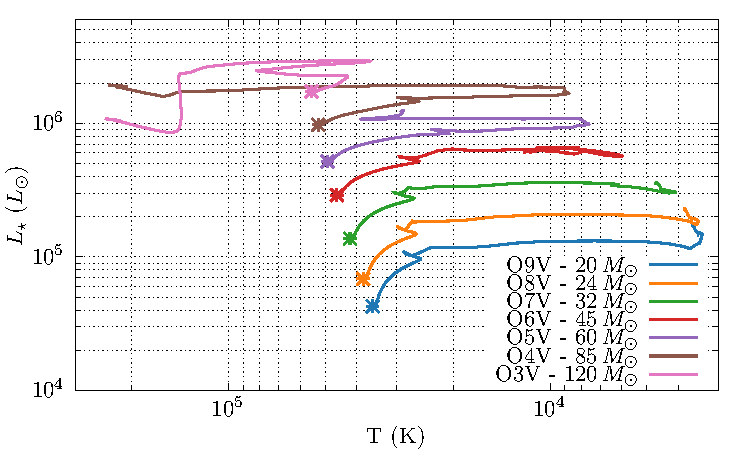
\includegraphics{assets/tracks/tracks.pdf}
  \caption[Stellar evolution tracks of massive stars]{Stellar evolution tracks of rotating O-type stars from the zero-age main sequence (ZAMS) to their end of life. Higher mass O-type stars undergo a significant increase in brightness and temperature as they evolve into LBV and then WR stars. The O3V star in particular appears to undergo two separate phases, clearly indicative of the high-mass case of Eq. \ref{eq:wrevolution}. The evolutionary tracks were derived from the MIST project \parencite{choiMesaIsochronesStellar2016,dotterMESAIsochronesStellar2016,paxtonModulesExperimentsStellar2011}.}
  \label{fig:mist-zams}
\end{figure}

% Lifespan 
The Wolf-Rayet phase only takes up a brief period of a typical massive stars lifespan, typically \SI{5e5}{\year}, or $\lesssim 10\%$ of the main sequence lifespan of a representative O-type star.
Despite this short lived phase, the Wolf-Rayet leaves a marked impact on the surrounding stellar environment through stellar feedback and in some cases interstellar dust production.

\subsubsection{The death of a star}

% Continued evolution, carbon burning
The star, still shedding a significant portion of its mass, continues its death march\footnote{I understand that this section has taken a flair for the dramatic, but what \emph{isn't} dramatic about the death of a star?}.
The core contracts further, heating to temperatures in the range of $10^9 \, \si{\kelvin}$, carbon atoms are smashed together and burned, producing many heavier elements:

\begin{equation}
  \begin{alignedat}{3}
    \atom{C}{12}{6} + \atom{C}{12}{6} & \rightarrow \atom{Ne}{20}{10} + \atom{He}{4}{2} && + \SI{4.62}{\mega\electronvolt} \\
    \atom{C}{12}{6} + \atom{C}{12}{6} & \rightarrow \atom{Na}{23}{11} + p && + \SI{2.24}{\mega\electronvolt} \\
    \atom{C}{12}{6} + \atom{C}{12}{6} & \rightarrow \atom{Mg}{23}{12} + n && + \SI{2.60}{\mega\electronvolt}
  \end{alignedat}
\end{equation}

\noindent
These reactions salvage miniscule amounts of energy per nucleon, burning through all carbon in the core in $\sim 10^3$ years.
% Neon burning, buildup of nuclear ash
The core continues to contract, more vigorous and less efficient fusion processes begin to pile up on each other.
The star burns neon, then oxygen, and then silicon -- the latter of which has a flurry of reaction modes that produce many different elements, and burns through the entire reserves in approximately a day
\parencite[Ch.~6]{ryanStellarEvolutionNucleosynthesis2010a}.

% Iron
Finally, iron begins to deposit in the core of the star.
All fusion processes at this point are endothermic.
Suddenly without any exothermic fusion processes -- and robbed of its only support mechanism against gravity -- the star rapidly collapses.
The core rushes in on itself, accelerating to a large fraction of the speed of light.
This collapse produces truly unimaginable densities and temperatures in excess of \SI{100}{\giga\kelvin}\footnote{I can state a temperature of \SI{100}{\giga\kelvin} but can you really \emph{imagine} it? Can anyone really comprehend that kind of temperature?} within the core; protons capture electrons, forming neutrons and emitting copious amounts of neutrinos.
Eventually neutron degeneracy suddenly halts the collapse, the near-relativistic core material suddenly rebounds and generates an enormous shock wave, causing the conditions inside the dying star to jump to more absurd temperatures and pressures.
The rebounding material forms a core collapse supernova, ejecting heavy elements formed through neutron capture into an unsuspecting universe.
What's left behind is a neutron star: the remnant of the electron capture mechanism from the original inward dive\footnote{Randall Munroe of \href{https://what-if.xkcd.com/73/}{\texttt{XKCD}} once stated a good description of supernovae that I like to tell people: ``However big you think supernovae are, they're \emph{bigger} than that.''} \parencite[Ch.~13]{longairHighEnergyAstrophysics2011}.

In the case of collapsing Wolf-Rayet stars and other supergiant evolved stars this can go even further.
Neutron degeneracy is insufficient to halt the collapse and the core collapses into a black hole.
The resultant jet of material from this hypernova\footnote{\emph{Bigger than bigger than that!}} makes up a gamma-ray burst (GRB), a phenomena that can threaten planets \emph{thousands} of light years from their point of origin.
We should stop here, this section was written to provide context as to what early-type stars fundamentally are: violent, destructive, and awe-inspiring.
It seems absurd that these systems could produce anything as fragile as interstellar dust.

And yet they \emph{do!}

\section{Interstellar Dust}
\label{sec:dust}

% Observational history
For much of the history of astronomy, interstellar dust was not its own field, nor was it studied in significant detail.
Instead it was regarded as nothing but a \emph{nuisance}.
Early astronomy relied solely on visible light observations, and at these wavelengths dust obscures dim and distant stars, as well as the innermost depths of the galaxy.
% Early astronomy, of course, was limited to the visible light spectra, at these wavelengths dust \emph{is} in fact a nuisance, contributing nothing and extincting stars and the innermost depths of the galaxy.
The first population counts of stars at the turn of the \nth{20} century were hampered by this extinction, with \textcite{kapteynAbsorptionLightSpace1909} noting:

\begin{quote}
  \textit{
    ``Undoubtedly one of the greatest difficulties, if not the greatest of all, in the way of obtaining an understanding of the real distribution of the stars in space, lies in our uncertainty about the amount of loss suffered by the light on its way to the observer.''
  }
\end{quote}

\noindent
The existence of dust grains was not considered until nearly a quarter of a century later, with research undertaken in 1930 by Robert J. Trumpler concluding that the observed interstellar reddening effect could only be accounted for by small grains of cosmic dust.
As technology progressed and non-visible astronomy became possible, we were for the first time able to peer past these obscuring clouds, bypassing them entirely.
The scientific community also found that the interstellar dust itself was interesting on its own, leading to further categorisation and parametrisation of these dust grains in the 1960's and 1970's
\parencite[4-13]{whittetDustGalacticEnvironment2002}.

Small grains of interstellar dust are a loose collective of atoms and molecules held together by weak molecular bonds, and are typically on the order of $10 \, \si{\angstrom}$ to $100 \, \si{\angstrom}$ in size.
These grains are formed from small, refractory dust cores around $5\,\si{\angstrom}$ across, in high density regions such as stellar atmospheres and dark interstellar clouds \parencite{spitzerPhysicalProcessesInterstellar2008}.
This initial accretion process can be quite rapid due to implantation of impinging carbon ions from the accompanying stellar wind \parencite{zubkoPhysicalModelDust1998a}.
While the largest dust grains can be on the order of centimetres (in the case of protoplanetary disks), the initial grain size that we use in this project is $50 \, \si{\angstrom}$.
There are a multitude of ways that these dust grains can grow and shrink in size, though only a few are simulated in this work.
This is due to either difficulty of implementation into our model or time constraints.
The first such mechanism for growth and destruction that will be discussed is grain-grain collision.
% Grain-grain interactions are the most easily understood, in regions with sufficiently high dust grain number densities, collisions can occur between the grains.
This interaction occurs in regions of high grain number densities and is dependent on the collision velocity between the grains, as well as the grain number density.
Low velocity collisions result in grain mergers, where these grains will stick together.
An initial attractive force through van der Waals interaction will occur, bringing the grains into contact.
Upon collision the contact area will deform and flatten, allowing for the grains to coagulate and merge.
Grain-grain coagulation occurs at very low velocities, typically $<\SI{100}{\metre\per\second}$, but this threshold velocity is typically lower for smaller, more tightly bound grains
\parencite{chokshiDustCoagulation1993}.
At higher collision velocities small grains can simply bounce off of each other, doing very little damage outside of mutual ablation of the grains.
At higher velocities still, grains can shatter and fragment each other.
In the case of high velocity shocks with large grains, this can result in the grains being completely pulverised, turning from an accretion process to the principle cause of dust destruction
\parencite{jonesGrainShatteringShocks1996,jonesDustDestructionProcesses2004}.

The most important method of destruction of dust for this project is grain-gas sputtering, this thermal interaction dominates dust destruction at all temperatures in shocks.
As an ion collides with a dust grain in a shock, the surface near the impact site is vaporised, this impact also drives a shock wave into the grain, which cause it to melt and shatter.
Over time material is ablated off of the dust grain, causing it to shrink in radius and eventually disintegrate.
% In order to simulate this we must simplify and parametrise this into a model, we start by assuming that the dust grain is spherical.
In the case of a spherical grain, as the gas collides with the grain, small amounts of it are vaporised and ejected from the surface, causing a reduction in grain radius, $a$, with a corresponding rate of radius change, $\dot a$.
This rate of radius change varies depending on the composition of the grain.
For instance, grains composed of ice would be more readily vaporised by impacts than sturdier grains composed of carbon or iron.
In this spherical case the dust destruction rate is also proportional to the number density of the gas, as the grain will be destroyed faster if there are more gas-grain interactions.

Calculating the exact dust sputtering yield incurred on a grain is a very complex process, requiring a summation of sputtering yields across all projectile ion species.
Instead, we use an approximation described by \textcite[Ch.~25]{drainePhysicsInterstellarIntergalactic2011} which significantly simplifies the process and does not require simulation of the dynamics of ions.
Between $10^5$ and $10^9$ Kelvin the following approximation is valid:


\begin{equation}
  \dot{a} \approx - \frac{1\times 10^{-6}}{1 + T_6^{-3}} \left(\frac{n\rms{H}}{\si{cm^{-3}}}\right) \si{\micro\metre\per\year},
\end{equation}

\noindent
where $T_6$ is the gas temperature in units of $10^6 \, \si{K}$.
The dust destruction rate is dependent on the grain temperature, rapidly reducing below $10^6\, \si{\kelvin}$, and is found to be roughly flat from \SI{1e6}{K} to \SI{3e8}{\kelvin} \parencite{tielens_physics_1994}.
We can therefore adopt a normalised grain lifespan $\tau\rms{gr}$, which we can use to calculate the dust destruction rate in our simulations:

\begin{equation}
  \tau\rms{gr} \equiv \frac{a}{\dot a} \approx \num{3e6} \frac{a}{n\rms{g}} \, \si{\year} , 
\end{equation}

\noindent
where $n\rms{g}$ is the gas number density \parencite{drainePhysicsDustGrains1979,dwekCoolingSputteringInfrared1996}.
The value of \SI{3e6}{\year} was chosen for this project as it is more typical of temperatures in the post-shock region of a WCR, between $10^6\,\si{\kelvin}$ and $10^7\,\si{\kelvin}$ (Fig. \ref{fig:grain-lifespan}).
How this destruction rate is implemented into the simulations for this project is discussed in more detail in Section \ref{sec:bidmas}.

\begin{figure}[h]
  \centering
  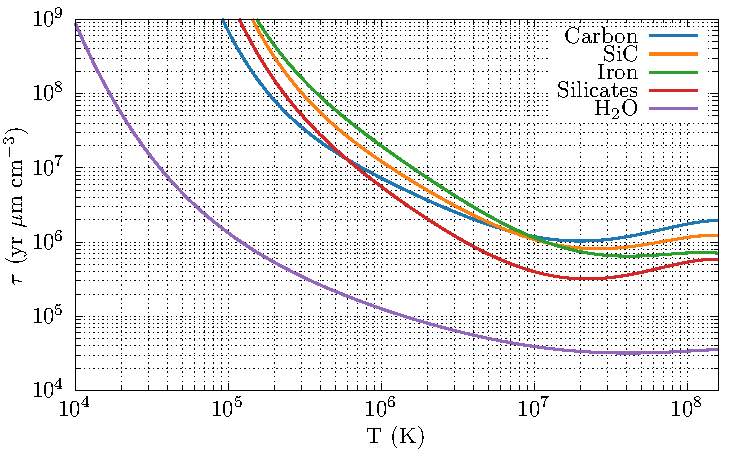
\includegraphics{assets/tielens-sputtering/sputter.pdf}
  \caption[Grain lifetime comparison]{Comparison of grain lifetimes for various interstellar dust species undergoing thermal sputtering in a fast interstellar shock. Lifetime is normalised to a grain radius of \SI{1}{\micro\metre} and a flow of \SI{1}{\gram\per\centi\metre\cubed} in a shock of solar abundance. Data is derived from \nth{5} order polynomial fits calculated in \textcite[Table~4]{tielens_physics_1994}.}
  \label{fig:grain-lifespan}
\end{figure}

% Dust-grain agglomeration 
At lower velocities gas can impact onto grains and stick to their surface.
This steady accretion process can be described in the form of another fairly efficient model.
By considering a spherical grain moving through a flow of atoms with a number density $n\rms{a}$, a certain number of these atoms would collide and stick to the dust grain, this sticking probability is defined as $\xi$.
This sticking factor is found to be $\approx 1$ for neutral atoms\footnote{Though we adopt a more conservative value of $0.1$ due to the turbulent nature of the environments that are studied in this project.} \parencite{watsonAbundancesInterstellarMolecules1972}.
Above a threshold velocity, atoms fail to adhere to the grain surface in significant quantities, and at even higher velocities contribute to the sputtering process instead \parencite{spitzerPhysicalProcessesInterstellar2008}.
For this research, this threshold temperature was defined as \SI{14000}{\kelvin}.

If we model a grain of radius $a$, the cross section, $\sigma$, of the grain moving through the gas would be $\sigma = \pi a^2$.
In the case of a grain moving through a gas of composition $x$ and density $\rho_x$ where the grain is significantly larger than the atoms composing the gas, it is found that the rate of change in the grain mass, $dm\rms{gr}/dt$, is:

\begin{equation}
  \frac{dm\rms{gr}}{dt} = \sigma w_{x} \rho_{x} = \pi a^2 \rho_{x} w_{x} \xi_{x} ,
\end{equation}

\noindent
where $w_x$ is the RMS velocity of the gas.
The associated rate of change in grain radius, $da/dt$, is found to be:

\begin{equation}
  \frac{da}{dt} = \frac{w_x \rho_x \xi_x}{4 \rho\rms{gr}},
\end{equation}

\noindent
where $\rho\rms{gr}$ is the bulk density of the dust grain.

A myriad of other dust destruction processes exist, such as electron-grain and cosmic ray-grain interaction.
However, these are considered to be out of the scope of this project, and not influential in the case of a hot gas or dense post-shock environment
\parencite{jonesDustDestructionProcesses2004}.
Outside of shocks, dominant destruction processes include thermal and photo-dissociation methods.
UV light emitted from stars can ionise atoms on the surface of the grain, ejecting them from the surface, slowly ``boiling'' material from the grain.
This of course makes the premise of our project all the more curious, with so many mechanisms underpinning dust destruction, particularly in hot, dense environments, how come we observe significant dust production in Wolf-Rayet binary systems?

\subsection{Dust composition}

% Grain types being considered, amorphous carbon grains
The only species of interstellar dust studied in this thesis are composited of carbon.
$sp^2$- (graphite) and $sp^3$-bonded (diamond) dust grains have been detected from their characteristic emission lines, as well as hydrocarbon chains and Polycyclic Aromatic Hydrocarbons (PAHs).
Complex organic molecules have also been detected in dusty environments, which are believed to have formed on the surface of dust grains, instead of forming within the ISM itself
\parencite{herbstComplexOrganicInterstellar2009}.
The primary dust detected in CWB systems is amorphous carbon grains, which are defined as grains with a mixture of $sp^2$- and $sp^3$-bonded carbon with no structural order or polymerisation
\parencite{draineInterstellarDustGrains2003}.
% Other grain types, PAHs, ice and silicates
Other species of interstellar dust are abundant throughout the ISM.
These species include water ice, as well as silicate and iron grains.
These grain species have not been detected in dust producing CWB systems.
Amorphous carbon grains are also markedly more resistant to erosion and fragmentation due to shocks than other grain types.
Amorphous grains are also more resistant to thermal sputtering, due to their higher sublimation temperature.
This resilience is vital if they are to survive in the extreme conditions of a CWB system
\parencite{draineDestructionMechanismsInterstellar1979}.

\subsection{The importance of interstellar dust}
\label{sec:dustimportance}

We should ask ourselves, why are dust grains important enough to merit so much time and effort from researchers?
Over this short section we will attempt to explain in brief why dust grains are so important.

% Interstellar dust grain species

Over 150 molecular species have been observed in the interstellar medium, with a surprisingly complex degree of organic chemistry; of the molecules with six or more atoms that have been detected, 100\% of these have been organic in nature.
Such complex organic molecules include benzene, acetone and ethanol, which are complex molecules that should not form in significant yields in interstellar gas-phase chemistry.
Instead, these organic species form on the surface of interstellar dust grains, with gas-phase chemistry accounting for simple molecule production such as $\text{H}_2$ and $\text{CO}$
\parencite{herbstComplexOrganicInterstellar2009}.
The role of dust as the chemical refineries of the interstellar medium has a number of effects when it comes to star and planetary formation, as well as organic and pre-biotic chemistry throughout the universe.
It is no understatement to say that the universe would be markedly different if interstellar dust was not so abundant.

% Coolant in collapsing gas clouds, stellar cycle
Dust grains are also vitally important in the star formation cycle.
As a giant molecular cloud (GMC) collapses, it heats up.
In an adiabatic case the increased temperature would provide a counterbalancing pressure on the collapsing cloud, forming a hydrostatic equilibrium and preventing the cloud from collapsing any further.
In the case of extremely massive clouds, this collapse can still occur as gravity will dominate, but this equilibrium dictates the minimum mass for a cloud to collapse into a protostar.
As such, for all but the most massive stars to form, energy must be lost in the form of radiation
\parencite{ward-thompsonIntroductionStarFormation2011}.
As cooling from dust grains is extremely efficient in cold, dense environments, this mechanism is well-suited for the environment of a GMC.
In addition to cooling through rotational mechanisms of simple molecules in the gas-phase of the medium, these processes sufficiently cool the GMC, allowing for further collapse.
In addition, dust grains would also provide a replenishing source of cooling molecules such as CO and OH through non-thermal grain desorption processes.
The presence of dust grains within a GMC therefore strongly influences the minimum mass of stars
\parencite{williamsChemistryCosmicDust2015}.

% Planetary formation
Interstellar dust is also important for planetary formation.
Collision between refractory dust grains is the first stage of planetesimal formation.
Within the protoplanetary disk, low velocity collisions between micron-sized grains can occur, causing these grains to stick and rapidly accrete.
If the local region of the disk is gravitationally unstable, these small grains will form a gravitationally bound cluster, and contract over time into a planetesimal.
Afterwards, rapid accretion of other planetesimals gives rise to the formation of both rocky planets and gas giants
\parencite{apaiProtoplanetaryDustAstrophysical2010}.
Dust is also a regulator of opacity, which determines the temperature structure and composition of the protoplanetary disk.
Finally, and perhaps most importantly to the reader, the complex organic molecules produced in the dust grain are pre-biotic precursors to life
\parencite{birnstielDustEvolutionFormation2016}.

As the role of interstellar dust in star and planet formation, as well as the long-term implications of the formation of life in the universe are \textit{slightly} out of the scope of this project, we will stop here, and move on to the topic of colliding stellar winds.

\section{Colliding Wind Binary Systems}
\label{sec:cwb}

Colliding wind binaries (CWBs), in opposition to all known laws of astrophysical nomenclature is an easy to understand term: it is a binary system wherein stellar winds undergo collision.
Unfortunately, the simplicity of the systems ends here, CWB systems are very poorly understood phenomena due to a variety of factors.

\subsection{History of CWB observation}

%History and classification, useful sources in Stevens & Pollock 1994 

Early observations beyond the visual spectrum led to the discovery of many new astrophysical phenomena.
One such discovery were extremely bright and variable thermal x-ray sources.
Many of these early galactic x-ray sources were found to be compact objects, and many more contained the characteristic spectral lines of a Wolf-Rayet star.
While single Wolf-Rayet stars are capable of producing x-rays if there are sufficient instabilities in the winds \parencite{gossetXMMNewtonLookWolfRayet2005}, this is typically much fainter (\cite{nazeNewXrayDetections2021}; typically $L\rms{x-ray} / L\rms{bol} < 10^{-7}$) than what was being observed from these systems
\parencite{sewardXraysEtaCarinae1979,oskinovaXrayEmissionSingle2015,rauwXrayEmissionMassive2022}.
The existence of CWB systems were independently proposed by \textcite{prilutskii_x_1976} and \textcite{cherepashchukDetectabilityWolfRayetBinaries1976}. 
Both research groups proposed that significant and variable x-ray flux would result from the collision between two stellar winds.
As these winds collide the gas becomes shocked and heated to temperatures on the order of \SI{1e8}{\kelvin} -- hot enough to emit an appreciable quantity of x-rays.
The x-ray variability can also be explained as a result of the orbital properties of the systems.
X-ray variability would result from the following effects:

% This may need to be expanded on or changed
\begin{itemize}
  \item Eccentricity in the orbits of the systems, leading to differing shock intensity and changing of the shock geometry, changing the fraction of the winds being shocked.
  \item Edge-on orbits resulting occlusion of x-rays by the stellar wind from each star. 
  \item Photospheric eclipses in the case of high inclination angles.
\end{itemize}

\noindent
Such effects could not be produced within a single star system \parencite{pittard_x-ray_1999}.
% Further research by \textcite{pollockEinsteinViewWolfRayet1987} also found that single WR stars were typically faint, with the brightest x-ray emitting WR stars being confirmed to within massive binaries.
WR+OB systems were also found to be the brightest of such objects, while OB+OB binaries with significant x-ray flux were observed, these were typically less luminous.
% Early work categorising, using gamma 2 vel and V444Cyg
Early work was more concerned with x-ray observation, in particular the systems $\gamma^2$ Velorum and V444 Cygni, which were noted in particular as prototypical CWB systems by \textcite{prilutskii_x_1976}.
% Analysis pollock 1987 determined binary systems\cite{pollockEinsteinViewWolfRayet1987} 
Later, infrared observations of these systems found another, more curious attribute: a significant infrared excess correlating to dust formation around these systems \parencite{williamsInfraredPhotometryLatetype1987}.
This will be discussed in more detail later in this section.
% , but needless to say this phenomena is puzzling, as fragile grains of interstellar dust would not survive for long in the outflow of a WC star, due to the high wind temperatures and immense UV flux.
% Because of this, dust growth was speculated, and later confirmed, to occur within the Wind Collision Region, the topic of the next section of this thesis.

\subsection{The Wind Collision Region}
\label{sec:wcr}

\begin{figure}[h]
  \centering
  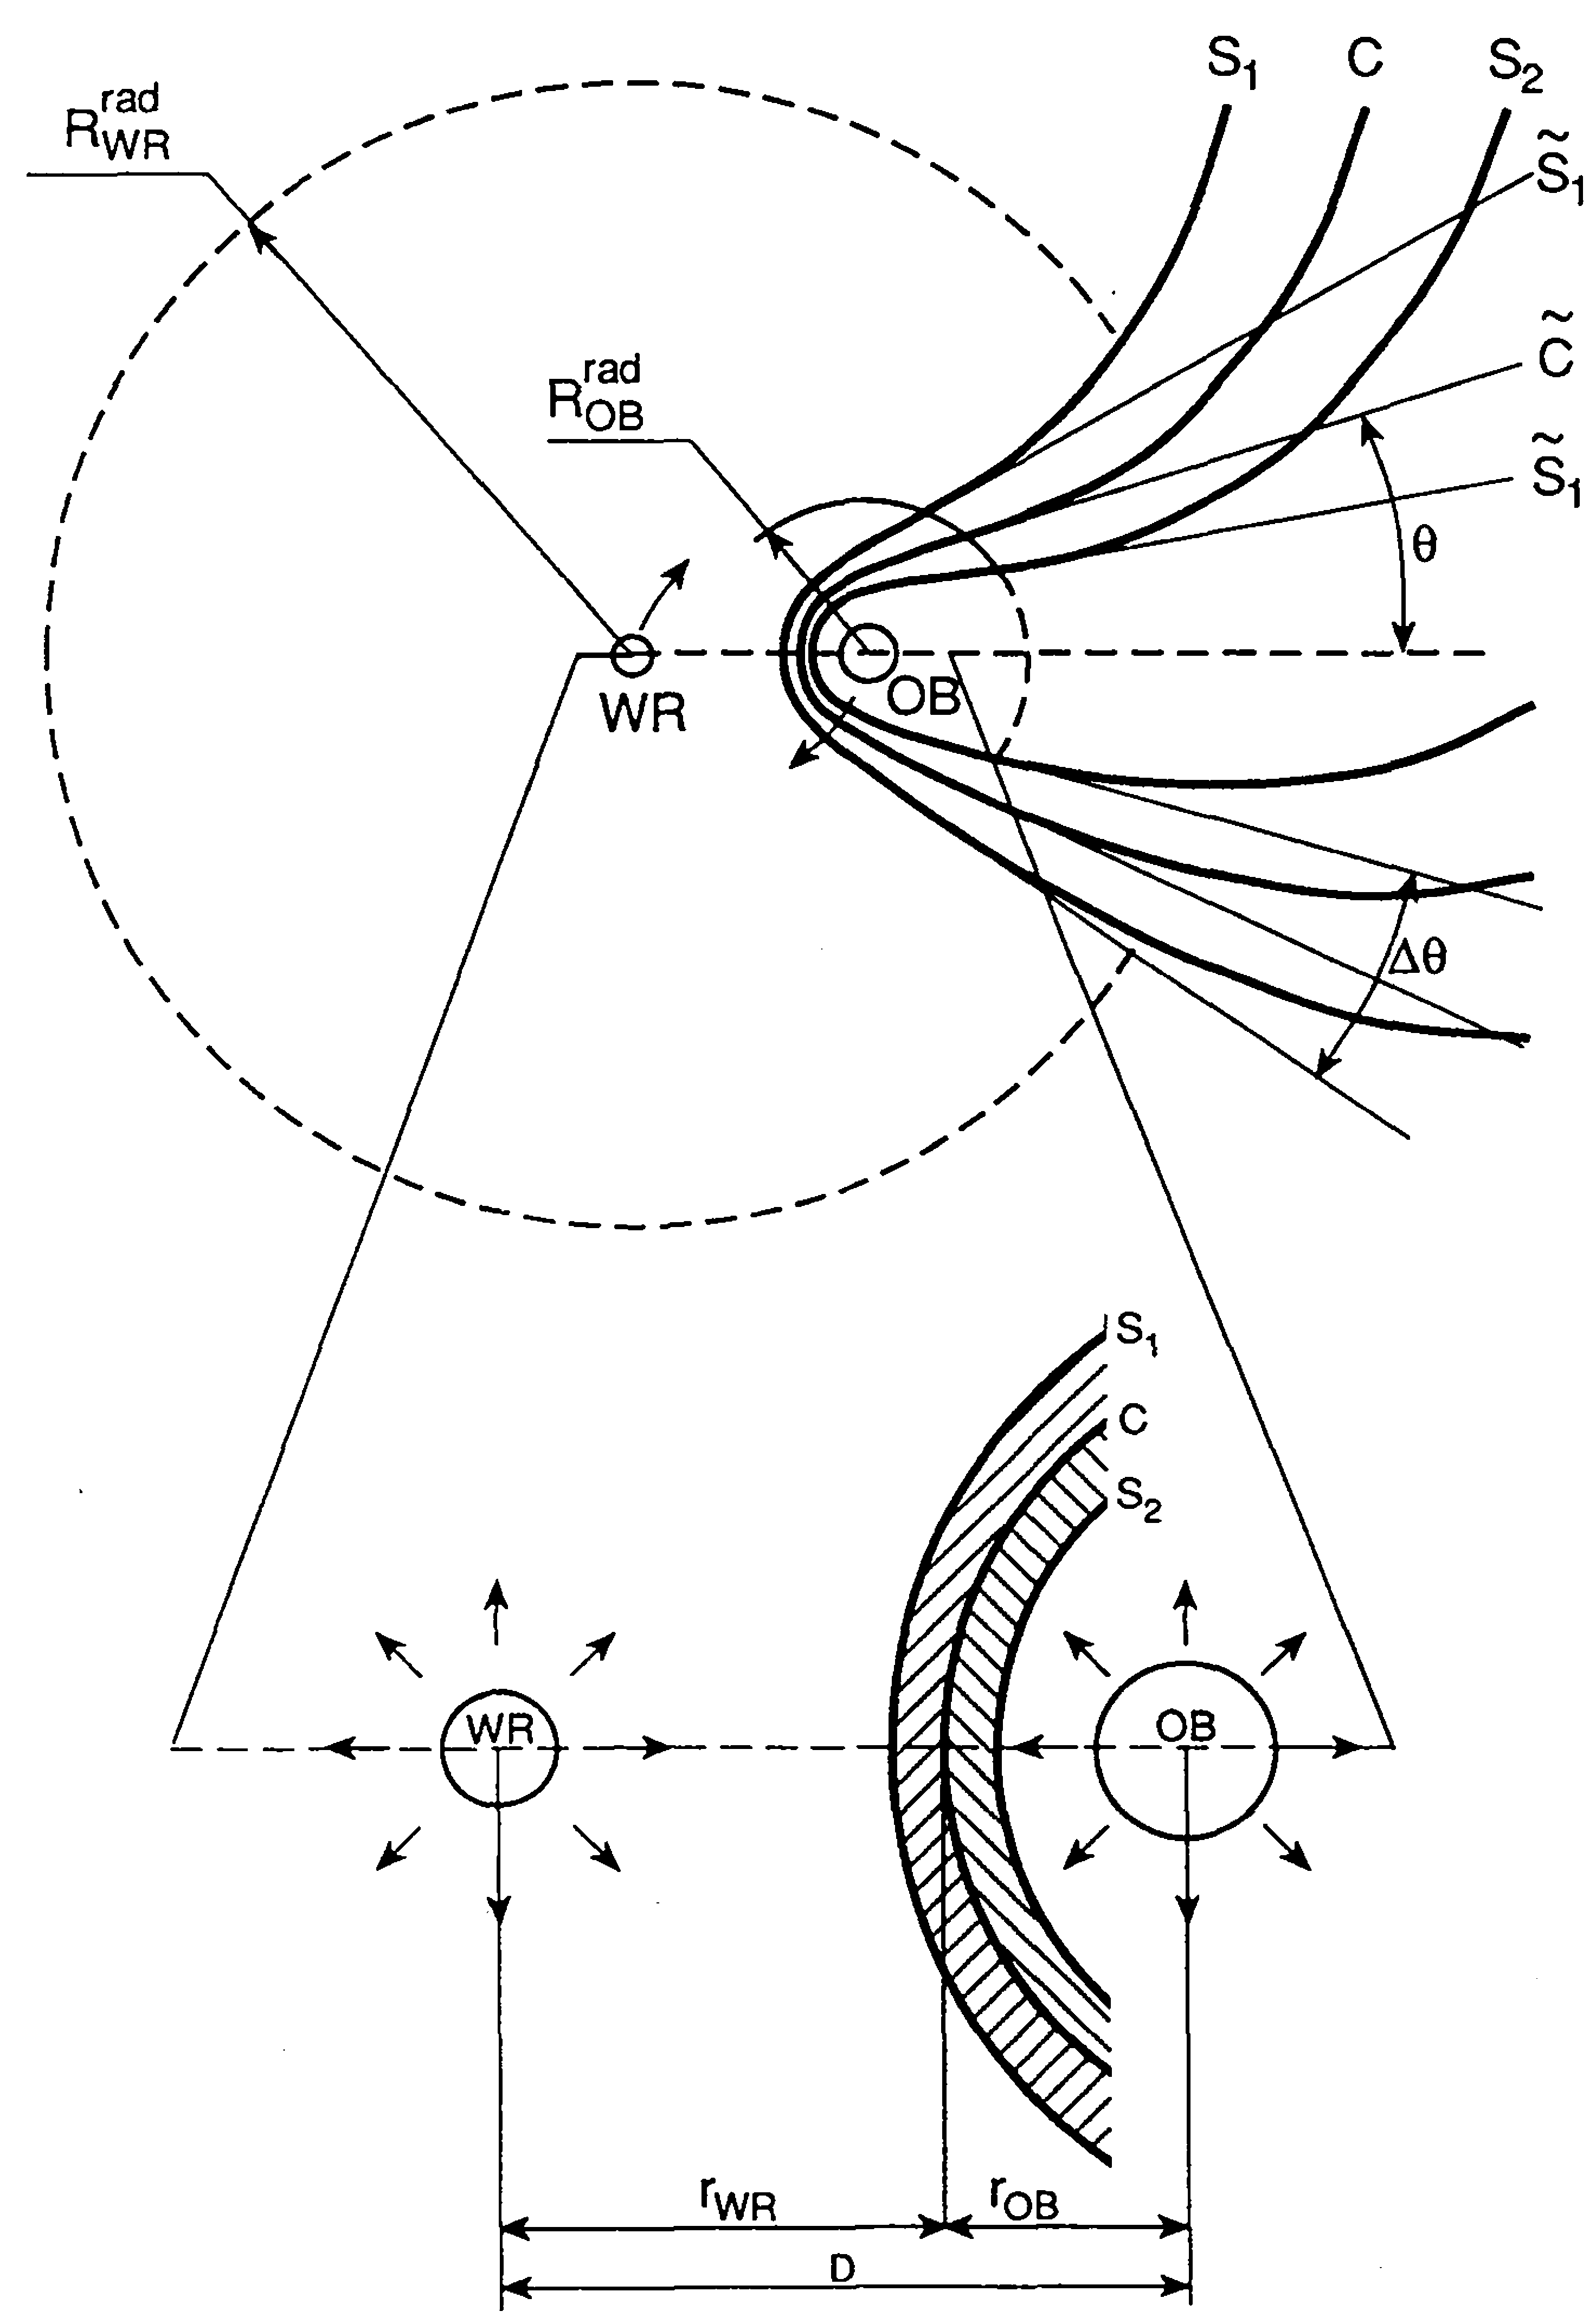
\includegraphics[width=3in]{assets/cwb-diagrams/eichler.png}
  \caption[\textit{A diagram of the Wind Collision Region \parencite{eichler_particle_1993}}]{A diagram of a typical Wind Collision Region inside a WR+OB CWB system. The $S_1$ and $S_2$ surfaces denote the shock waves from the primary and secondary winds respectively, and $C$ denotes the contact surface. The surfaces $\widetilde{S}_1$, $\widetilde{S}_2$ and $\widetilde{C}$ represent conic approximations of their corresponding surfaces at intermediate distances from the OB star. The region of stellar wind collision is hatched in the bottom diagram \parencite{eichler_particle_1993}.}
  \label{fig:wcr-diagram}
\end{figure}

\begin{figure}[h]
  \centering
  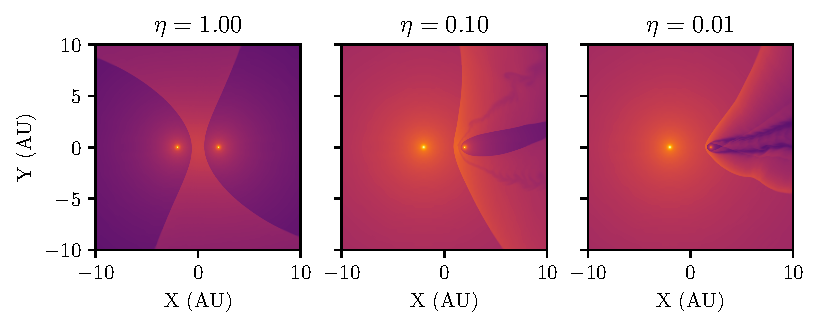
\includegraphics{assets/cwb-structure/ch1-eta-rho.pdf}
  \caption[Comparison of wind momentum ratio, $\eta$, on WCR structure]{Comparison of the WCR structure of CWB systems with wind momentum ratios of \num{1}, \num{0.1} and \num{0.01}. Momentum ratio is varied by changing the mass loss rate of the second star, $\dot{\text{M}}_2$. As $\eta$ decreases, the WCR begins to wrap itself around the secondary star. Orbital effects are also shown in this example.}
  \label{fig:wcr-eta}
\end{figure}

% What is this region
\noindent
The wind collision region (WCR) is the most violent and turbulent region of a CWB system, a region of high gas density and even higher temperatures.
If the interacting stellar winds are dense as they begin to interact, a shocked region of plasma in excess of \SI{1e8}{\kelvin} is formed, the winds rapidly decelerate from hypersonic to subsonic, liberating an enormous amount of mechanical energy, on the order of \SI{1e3}{\solarluminosity}.
This is the engine that drives the significant x-ray flux observed by astronomers in the 1970s, as well as other thermal and non-thermal emissions from radio waves to gamma rays
\parencite{eichler_particle_1993,grimaldoProtonAccelerationColliding2019}.
As a wind enters from either side of the wind collision region, it passes through a shock wave, and flows towards the centre of the wind collision region at the contact discontinuity, $C$ (Fig. \ref{fig:wcr-diagram}), and downstream of the system.
The post-shock wind is driven by a combination of thermal pressure from the outflowing stellar wind, as well as the significant momentum the wind carried had pre-shock \parencite{stevens_colliding_1992}.

The geometry of the WCR is influenced strongly by the wind parameters of both stars, the most important of which is the wind momentum ratio, or $\eta$, which we define as:

\begin{equation}
  \eta = \frac{\dot M_\text{OB} v^\infty_\text{OB}}{\dot M_\text{WR} v^\infty_\text{WR}},
\end{equation}

\noindent
where $\dot{\text{M}}_\text{WR}$ and $v^{\infty}_\text{WR}$ denotes the mass loss rate and wind terminal velocity of the primary (typically WR) star and $\dot{\text{M}}_\text{OB}$ and $v^{\infty}_\text{OB}$ denotes the mass loss rate and wind terminal velocity of the (typically OB) partner \parencite{usov_stellar_1991}.
A lower value of $\eta$ indicates a more unbalanced wind, with a wind momentum ratio of \num{0.01} or lower being common for a typical WR+OB system.
Additionally, if $\eta = 1$, we observe a sheet of interacting plasma flowing away from the system perpendicular to the orbital plane.
In the case of a typical system where the WR stars momentum is significantly larger than OB's, we observe the WCR extend and envelop the OB star, forming an approximately conical surface extending away from the Wolf-Rayet star (Fig. \ref{fig:wcr-eta}).


As the wind becomes more and more imbalanced, the contact discontinuity moves closer to the OB partner.
The position of this discontinuity can be predicted with the equation

\begin{equation}
  r_\text{WR} = \frac{1}{1+\eta^{1/2}} d_\text{sep} , ~~~ r_\text{OB} = \frac{\eta^{1/2}}{1+\eta^{1/2}} d_\text{sep} ,
\end{equation}

\noindent
where $r\rms{WR}$ is the distance from the WR star to the contact discontinuity, $r_\text{OB}$ is the distance from the OB star to the contact discontinuity and $d_\text{sep}$ is the orbital separation distance of the stars.
We can also approximate the opening angle, $\theta_c$, of the WCR using the equation provided by \textcite{eichler_particle_1993}

% Conic approximation
\begin{equation}
  \theta_c \simeq 2.1 \left(1 - \frac{\eta^{2/5}}{4}\right) \eta^{-1/3}, ~~ \text{for } 10^{-4} \leq \eta \leq 1. \label{eq:conic}
\end{equation}

% Wind shock factor, see Julians paper

% Analytical expressions of the opening angle for the shocks $S_1$ and $S_2$ have been provided by \textcite{pittardCollidingStellarWinds2018}.
% In this paper, a series of hydrodynamical simulations were performed with varying values of $\eta$, 
% The opening angle for $C$ was found to be consistent with the solution provided by \textcite{eichler_particle_1993}, while 

\noindent
Work by \textcite{pittardCollidingStellarWinds2018} on determining the accuracy of opening angle expressions such as equation \ref{eq:conic} found that this approximation is accurate under the condition $\eta > 0.01$, but begins to diverge significantly if this condition is exceeded.
This was accomplished through a series of hydrodynamical simulations with different values for $\eta$, with the resultant opening angle calculated from the fully advected simulations.
This work goes on to derive analytical solutions to the opening angles of the conic approximations of $\widetilde{S}_1$ and $\widetilde{S}_2$.
These solutions were found to be:

\begin{subequations}
  \begin{align}
    \theta_1 & = 2 \tan^{-1} \left(\eta^{1/3}\right) + \delta \theta , \\
    \theta_2 & = 0.658 \log_{10} \left(71.7 \eta \right) ,
  \end{align}
\end{subequations}

\noindent
where $\delta \theta$ is the opening angle of the WR shock in the limit that $\eta = 0$ (found to be $\delta \theta \approx \pi/9$).
From these estimations the fraction of each wind that is shocked, $f$, can be calculated:

\begin{subequations}
  \label{eq:windshockfraction}
  \begin{align}
    f_1 & = \frac{1 - \cos\left(\theta_1\right)}{2} , \\
    f_2 & = \frac{1 + \cos\left(\theta_2\right)}{2} .
  \end{align}
\end{subequations}

\noindent
\textcite{pittardCollidingStellarWinds2018} observed that the entirety of the secondary wind was shocked if $\eta \lesssim 0.014$, while in the typical wind momentum ratio regime $0.001 \leq \eta \leq 0.01$, only $\sim 10\%$ of the WR wind is shocked (Fig. \ref{fig:wind-shock-factor}).
While useful for describing the geometry of WCR in broad strokes, these equations are based on adiabatic simulations with instantaneous acceleration, and thus have their limitations.

\begin{figure}[ht]
  \centering
  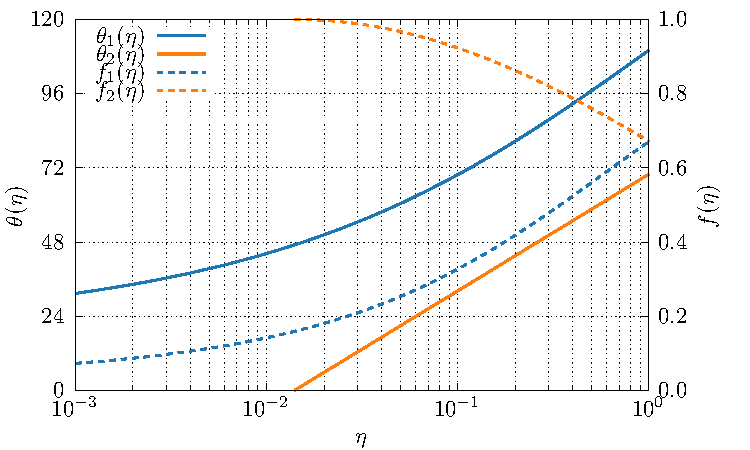
\includegraphics{assets/wind-shock-factor/shock-factor.pdf}
  \caption[Wind shock fraction, as a function of $\eta$]{Comparison of the opening angle of $\widetilde{S}_1$ and $\widetilde{S}_2$ as a function of $\eta$. The wind shock fraction, $f$, is also plotted. $\approx 10\%$ of the primary wind is shocked under typical WR+OB conditions, while the entire secondary wind is typically shocked.}
  \label{fig:wind-shock-factor}
\end{figure}

% Influence of orbital motion
Orbital motion is a significant factor in the geometry of a WCR.
As the stars orbit each other and the WCR curves and wraps around the system, the angle of the WCR relative to the outflow from the system is constantly changing.
The conical approximation as described in \textcite{eichler_particle_1993} was found to be valid to a distance of $r_\text{OB} \ll r \ll (P v^\infty_\text{WR})/2$, where $P$ is the orbital period.
In systems with a short orbital period, this can result in the production of a pinwheel-like structure as the WCR extends away from the stars.
For example, the systems WR104 and WR98a produce easily observable pinwheel structures, especially in the infrared.

\subsection{Cooling in the WCR}
\label{sec:wcrcooling}
%//TODO clean up this caption
%//TODO remove grid from plot
\begin{figure}[h]
  \centering
  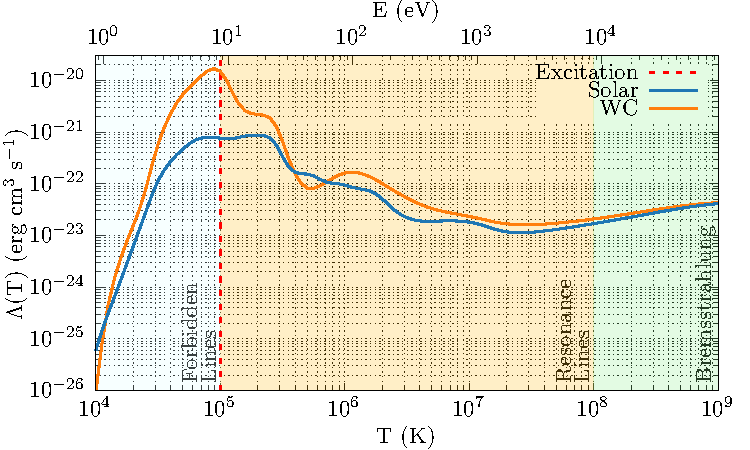
\includegraphics{assets/cooling-breakdown/cooling-curve-solar-withev.pdf}
  \caption[WC \& solar abundance plasma cooling curves]{Normalised plasma cooling rates as a function of temperature and thermal energy for solar abundance and WC abundance winds. The regions where forbidden line, resonance line and bremsstrahlung emission are dominant are highlighted, with H ionisation and recombination occuring between the forbidden and resonance line sections at $10^5$ \si{\kelvin}.}
  \label{fig:wcsolcooling}
\end{figure}

\begin{table}[h]
  \centering
  \begin{tabular}{lll}
  \hline 
  Temperature range & Dominant process & Spectral region \\
  \hline
  $T < 10^3 \, \si{\kelvin}$ & Molecular cooling & IR \\
  $\SI{5e3}{\kelvin} \lesssim T \lesssim \SI{1e5}{\kelvin} $ & Forbidden lines & \SI{21}{cm}, IR, Optical \\
  $T \approx \SI{1e5}{\kelvin}$ & H excitation/ionisation & Optical, UV \\
  $\SI{5e5}{\kelvin} \lesssim T \lesssim \SI{1e8}{\kelvin} $ & Resonance lines & Far UV, soft x-ray \\
  $T \gtrsim \SI{1e8}{\kelvin} $ & Bremsstrahlung & Radio \\ \hline
  \end{tabular}
  \caption[Cooling processes at various temperature ranges]{Breakdown of dominant cooling processes at various temperature ranges from \textcite[Ch.~6]{dysonPhysicsInterstellarMedium2021}. Whilst H excitation/ionisation occurs over a very short temperature range, it is extremely influential, causing a global peak in the cooling rate at $\approx 10^5$ \si{\kelvin}. These temperature ranges are depicted in Fig. \ref{fig:wcsolcooling}.}
  \label{tab:coolprocess}
\end{table}

% Whilst we have described the dynamics and structure of the post-shock WCR, we have not described the temperatures.
Such violent regions of space are \emph{exceedingly} hot.
In a fixed frame of reference, the immediate post-shock temperature, $T\rms{s}$, is calculated via the formulae:

\begin{equation}
  T\rms{s} = \frac{3\mu m\rms{H}}{16 k\rms{B}} V\rms{s}^2 ,
\end{equation}

\noindent
where $\mu$ is the mean molecular mass, $k\rms{B}$ is the Boltzmann constant\footnote{\SI{1.381e-16}{erg.K^{-1}}}, and $V\rms{s}$ is the shock velocity
\parencite[Ch.~9]{macielHydrodynamicsStellarWinds2014}.
For stellar winds colliding with a relative velocity of \SI{2000}{\kilo\metre\per\second} we find that the immediate post-shock temperature is of the order $10^8\,\si{K}$.

But how does the WCR cool to temperatures suitable for dust formation?
Dust destruction occurs readily at temperatures $>10^6\, \si{\kelvin}$, with temperatures $<10^4\,\si{\kelvin}$ being conducive to dust formation.
Furthermore, this cooling has to be very rapid, as observations have shown that the bulk of dust formation occurs $\lesssim \SI{100}{\au}$ from the point of initial shock.
In fact, winds moving at velocities in excess of \SI{1000}{\kilo\metre\per\second} would clear this distance in less than half a year!
In an adiabatic shock, we would find that the gas cools purely through expansion in accordance with the ideal gas law; as the flow from the WCR begins to spread away, it cools on an extremely slow timescale.
Gas and plasma within the gas are subject to a variety of cooling mechanisms, which contribute to removing energy from the medium.
As atoms and ions are excited by collisions or photons, the particles are excited to higher energy levels, releasing photons and de-exciting to their ground state.
These photons can leave the medium, and in dense mediums this can occur over multiple adsorption/re-emission events.
This causes the photon to leave the gas through a ``random walk'' which is dependent on the wavelength of the photon and the density of the gas.
% If the gas is sufficiently dense, the energy can be removed quite rapidly, with collisional energy effectively coupled to this photon emission, this results in a drop in temperature.
Inversely, if the post-shock WCR is sufficiently dense, ionising radiation from the parent stars cannot penetrate deep into the WCR, protecting dust grains and preventing heating aside from a small contribution from galactic cosmic rays (GCRs).

Strong radiative cooling results in much higher compression levels of the post-shock gas than the adiabatic limit of $\rho\rms{post-shock} = 4\rho\rms{pre-shock}$.
This is crucial to the formation of dust in the post-shock region, which relies on high densities as well as cool temperatures (this is explored further in Section \ref{sec:cwbdust}).

The influence of each cooling mechanism varies over a particular temperature range, due to the collision energy of the atoms and ions.
While there is some overlap, certain mechanisms are clearly dominant over specific temperature ranges (Table \ref{tab:coolprocess} and Fig. \ref{fig:wcsolcooling}).
In the ``warm\footnote{See what I mean about the phrase ``warm''?}'' phase we find that forbidden line emission through atomic hydrogen or metallic ions is dominant, while at higher temperatures higher energy processes such as H recombination and resonance line emission dominate.
At extremely high temperatures in the immediate post-shock WCR, free-free processes such as bremsstrahlung dominate
\parencite[Ch.~6]{dysonPhysicsInterstellarMedium2021}.
In this section we will discuss these primary mechanisms of cooling.

\subsubsection{``Cool'' medium}

At temperatures from 10 to $10^3 \, \si{\kelvin}$ atomic excitation is extremely unlikely, other than heating events from adsorption of cosmic rays.
Instead, spontaneous rotational and vibrational transitions in molecules shed what little thermal energy remains in these clouds.
The most influential molecules on the temperature of these gas clouds are $\text{H}_2 \text{O}$, $\text{H}_2$ and $\text{CO}$
\parencite{neufeldRadiativeCoolingWarm1993,neufeldThermalBalanceDense1995}.
Through molecular transitions for cooling and heating through cosmic rays, a stable temperature in the order of \SI{10}{\kelvin} is maintained in these cold, dense clouds.
While this mechanism is essential for understanding how molecular clouds remain so cool, heating from the parent stars will prevent the WCR from getting this cold.

\subsubsection{``Warm'' medium}

% Section on forbidden line emission
Between $10^4$ and $10^5 \, \si{\kelvin}$, radiative cooling is dominated by forbidden line transitions\footnote{Like many other phenomena discussed in this thesis, this too is a misnomer. This transition was initially believed to be prohibited under contemporary models of atomic physics. This is in fact just astrophysicists jumping the gun again!}.
This mechanism releases energy through a hyperfine splitting of the $1s$ ground state of hydrogen, where the hydrogen atom spontaneously emits photons de-excite to a more stable spin state.
Transition between a proton/electron parallel ($\uparrow\uparrow$) to antiparallel ($\uparrow\downarrow$) spin state emits a photon of energy \SI{5.86}{\micro\electronvolt}:

\begin{figure}[H]
  \adjustbox{scale=0.6,center}{%
    \begin{tikzcd}
      {\text{p}^\uparrow \text{e}^\uparrow} &&& {} & {S=1,~g_u=3} \\
      &&& {} && {\lambda=21\, \text{cm}} \\
      {\text{p}^\uparrow \text{e}^\downarrow} &&& {} & {S=0, ~ g_u = 1} \\
      &&& {}
      \arrow[no head, from=1-1, to=1-5]
      \arrow[shorten >=3pt, from=1-4, to=3-4]
      \arrow[no head, from=3-1, to=3-5]
      \arrow[color={rgb,255:red,214;green,92;blue,92}, squiggly, from=2-4, to=2-6]
    \end{tikzcd}
  }
  \caption[The \SI{21}{cm} spectral line]{Energy level diagram of the \SI{21}{cm} spectral line -- an all-in-one galactic yard stick, stopwatch and cooling mechanism.}
  \label{fig:quiver-h}
\end{figure}

\noindent
Despite the parallel spin state being metastable, with a very long lifetime of \SI{11}{\mega\year}, it occurs extremely readily in a large volume of gas in the ISM.
Gas at this temperature is relatively transparent to radio waves, and as such the \SI{21}{cm} line can steadily remove energy through cooling\footnote{In the fighting game community (FGC), this is referred to as ``chip damage''.}.
Due to the presence of enormous quantities of atomic hydrogen, the \SI{21}{\centi\metre} line is one of the most prevalent type of radio emission in the galaxy\footnote{In fact, the wavelength and parallel spin state actually make up a set of fundamental units used in messages such as the \textit{Voyager} and \textit{Pioneer} messages due to its ubiquity.}
\parencite[Ch.~8]{drainePhysicsInterstellarIntergalactic2011}.
In winds with a higher metallicity, forbidden line transitions from ions with more electron orbitals, can become dominant.
Such ions include $\text{O}^+$ and $\text{O}^{++}$:

\begin{figure}[H]
  \adjustbox{scale=0.6,center}{%
    \begin{tikzcd}
      {} &&&&& {^2 \text P_{1/2}} &&&& {} & {} &&&& {^1 \text S_0} \\
      {} &&&&& {^2 \text P_{3/2}} &&&&& {} &&&&&& {\lambda = 436.3 \, \text{nm}} \\
      &&&&&&&&& {} & {} & {} & {} && {^1 \text D_2} \\
      {} && {} &&& {^2 \text D_{3/2}} &&&&&& {} &&&&& {\lambda = 500.7 \, \text{nm}} \\
      {} &&& {} && {^2 \text D_{5/2}} &&&&&& {} & {} &&&& {\lambda = 495.9 \, \text{nm}} \\
      && {} &&&&& {\lambda = 372.6 \, \text{nm}} && {} && {} &&& {^3 \text P_2} \\
      &&& {} &&&& {\lambda = 372.9 \, \text{nm}} && {} &&& {} && {^3 \text P_1} \\
      {} && {} & {} && {^4 \text S_{3/2}} &&&& {} &&&&& {^3 \text P_0}
      \arrow[no head, from=4-1, to=4-6]
      \arrow[no head, from=5-1, to=5-6]
      \arrow[no head, from=8-1, to=8-6]
      \arrow[from=4-3, to=8-3]
      \arrow[from=5-4, to=8-4]
      \arrow[draw={rgb,255:red,214;green,92;blue,92}, squiggly, from=6-3, to=6-8]
      \arrow[draw={rgb,255:red,214;green,92;blue,92}, squiggly, from=7-4, to=7-8]
      \arrow[no head, from=8-10, to=8-15]
      \arrow[no head, from=7-10, to=7-15]
      \arrow[no head, from=6-10, to=6-15]
      \arrow[no head, from=1-10, to=1-15]
      \arrow[from=1-11, to=3-11]
      \arrow[from=3-12, to=6-12]
      \arrow[from=3-13, to=7-13]
      \arrow[draw={rgb,255:red,214;green,92;blue,92}, squiggly, from=4-12, to=4-17]
      \arrow[draw={rgb,255:red,214;green,92;blue,92}, squiggly, from=2-11, to=2-17]
      \arrow[no head, from=3-10, to=3-15]
      \arrow[no head, from=2-1, to=2-6]
      \arrow[no head, from=1-1, to=1-6]
      \arrow[draw={rgb,255:red,214;green,92;blue,92}, squiggly, from=5-13, to=5-17]
    \end{tikzcd}
  }
  \caption[$\text{O}^{+}$ and $\text{O}^{++}$ spectral line transitions]{Forbidden line transitions in the $\text{O}^{+}$ (left) and $\text{O}^{++}$ (right) ground states.}
  \label{fig:quiver-oplus}
\end{figure}

\noindent
These transitions release significantly more energy, and as such are a more efficient way of removing energy from metal enriched winds, explaining the increase in cooling rate in the WC abundance wind in Fig. \ref{fig:wcsolcooling}
\parencite[Ch.~5]{dysonPhysicsInterstellarMedium2021}.
As the temperature increases, the rate of cooling peaks.
In WCRs containing hydrogen this is consistent with recombination of electrons and hydrogen ions, releasing photons of energy $13.6\,\si{\electronvolt}$.

\subsubsection{``Hot'' medium}

Beyond $10^6\,\si{\kelvin}$\footnote{Which we have arbitrarily defined as ``hot''.} forbidden line transitions are no longer dominant as metastable levels in the ground state of ions become increasingly rare as the species become more and more ionised ($\text{C}^{3+}$, $\text{O}^{4+}$ etc.).
Instead, resonance line transitions in metals, the driving force behind the stellar winds, begin to take over the role of cooling.
These lines are not metastable like forbidden lines, and have much higher transition probabilities.
As such, the emission rate is still quite high, but is constantly decreasing as temperature increases, as the probability for an ion being completely ionised increases.
At temperatures in excess of $10^7\,\si{\kelvin}$, even these heavier ions are completely ionised.
With their electrons stripped bare they simply do not have any resonance lines left!
However, at these extreme temperatures, the WCR is cooled through radiation emitted via the bremsstrahlung\footnote{Or ``braking radiation'' if you have forgotten how to spell bremsstrahlung.} mechanism.
This mechanism is comparatively simple: as the path of a high velocity charged particle is changed, it emits radiation equivalent to the change in velocity, in accordance with the conservation of energy.
As this process is not determined by emission lines or energy levels, it increases with temperature, as stronger deflections release higher energy photons.
Therefore, this process acts as the dominant cooling process in the universe at temperatures beyond $10^9 \, \si{\kelvin}$
\parencite[Ch.~6]{longairHighEnergyAstrophysics2011}.

\subsubsection{Radiative effects in WCRs}

% Temperature range, temperature importance
CWB systems are interesting interstellar phenomena.
There are only a handful of phenomena in space that operate on such a large temperature range over such a short timespan.
These systems are highly dependent on the temperature, and therefore very dependent on the amount of cooling occurring in the system.
% Slight discussion on difficulty of simulation
This can present tremendous challenges trying to simulate them, due to the difficulty of calculating contributions to cooling.
Simulating cooling can significantly impact the stability of the simulations, which are already hard enough to perform on their own.
% Quick discussion on how we do it in the simulation, but nothing to extreme, link to appropriate section
The first problem is solved by pre-calculating the emission rate of gas with a specific metallicity over a range of temperatures.
This is accomplished using models such as the Mewe-Gronenschild-Kaastra (\texttt{MEKAL}) model, and incorporating the output of these models into the simulation in the form of a lookup table
\parencite{meweCalculatedXradiationOptically1985,kaastraSPEXHighresolutionCosmic2013}.

% Introduce Lambda, fundamental value for cooling
In order to explore the contribution of cooling to the structure of the WCR, we must do what many\footnote{But possibly not \emph{all}.} astrophysicists despise the most: describe something mathematically.
First, in order to determine the amount of cooling occurring at a particular temperature, we summate the contributions of all energy loss mechanisms -- from forbidden lines to bremsstrahlung -- into a single value.
We first define the energy loss rate of a volume of gas, $\mathcal{L}(T)$, which in the case of plasma cooling is calculated by the equation

\begin{equation}
  \label{eq:energylossrate}
  \mathcal{L}(T) = \left(\frac{\rho}{m\rms{H}}\right)^2 \Lambda(T) = n\rms{g}^2 \Lambda(T) , 
\end{equation}

\noindent
where $n\rms{g}$ is the number density of the gas and $\Lambda(T)$ is the emissivity of the gas \parencite{stevens_colliding_1992}.
This assumes that the photons produced will eventually leave the gas.
As we can see, the rate of cooling in a gas is proportional to the square of the number density; as the density of the post-shock flow increases, it cools faster, despite having more internal energy.
Other methods of cooling and heating are not as strongly dependent on the number density of the gas.
For instance, dust cooling, which we will discuss later, has a dependence of $\mathcal{L}\rms{d} \propto n\rms{g}$, while cosmic ray heating has a dependence of $\mathcal{L}\rms{CR} \propto n\rms{g}^{-1/2}$ \parencite{wienerCosmicRayHeating2013}.

Cooling becomes influential on the system if gas in the WCR is able to sufficiently cool before it can leave the WCR.
To describe this \textcite{stevens_colliding_1992} introduced the wind cooling parameter, $\chi$, which is the ratio of the cooling time, $t\rms{cool}$, and the shock region escape time, $t\rms{esc}$:

\begin{equation}
  \chi = \frac{t\rms{cool}}{t\rms{esc}}.
\end{equation}

\noindent
If we determine the cooling time as the amount of time required for the gas to radiate \emph{all} of its energy, we find that

\begin{equation}
  \label{eq:taucool}
  t\rms{cool} = \frac{e}{\mathcal{L}(T)} = \frac{3}{8} \frac{k\rms{B} T}{n\rms{g} \Lambda(T)},
\end{equation}

\noindent
where $e$ is the internal energy per unit volume of the gas.
This value is appropriate in the case of a strong shock with a ratio of specific heats of $\gamma = 5/3$.
The escape timescale can be approximated with the equation

\begin{equation}
  \label{eq:tauesc}
  t\rms{esc} = \frac{d\rms{sep}}{c\rms{s}},
\end{equation}

\noindent
where $c\rms{s}$ is the sound speed.
\textcite{stevens_colliding_1992} describes an equation to approximate $\chi$ for each wind, which is used throughout this thesis:

\begin{equation}
  \label{eq:coolingparameter}
  \chi \approx \frac{v_{\infty,8}^4 d\rms{12}}{\dot{\text{M}}_{-7}},
\end{equation}

\noindent
where $v_{\infty,8}^4$ is the wind terminal velocity in units of $10^8 \, \si{cm.s^{-1}}$, $d\rms{12}$ is the orbital separation distance between the stars in units of $10^{12} \, \si{cm}$ and $\dot{\text{M}}_{-7}$ is the mass loss rate of the star in units of $10^{-7} \, \si{\solarmass\per\year}$.

In the case of a star with a cooling parameter of $\chi \gg 1$, the resultant stellar wind behaves adiabatically in the post-shock environment, producing a smooth flow.
As $\chi$ decreases and approaches 1, the post-shock wind is increasingly dominated by its radiative processes.
The stars post-shock wind is assumed to be dominated by radiative processes if $\chi \leq 1$.
In this case the gas cools rapidly after being shocked, leading to the formation of thermal instabilities.
This is seen in Fig. \ref{fig:chicomparison}, which compares a series of simulations with a wind momentum ratio of $0.02$ and an increasing separation distance.
As $\chi\rms{WR}$ decreases we see that the WCR shows clear signs of thermal instability, and an increasingly turbulent wind, in line with the predictions made in the equation.
Instabilities can also be produced by other mechanisms, such as KH instabilities, through imbalanced wind velocities.

Based on this equation we can now infer that winds that are strongly radiative in the post-shock WCR environment are both slow\footnote{Comparatively, of course, we still observe winds travelling at almost 1\% of $c$!} and dense.
Therefore, we can infer that typically the WR stars wind behaves radiatively, while the OB star in a CWB system behaves adiabatically.
Variability of $\chi$ can occur over a comparatively short timescale to the lifespan of the star due to the $\chi \propto d\rms{sep}^{-1}$ dependency.
Whilst variation of $\vinf$ and $\mdot$ for each wind will not vary significantly over the timescale of a single orbit, in the case of CWB systems with a highly eccentric orbit, the change in separation distance can cause $\chi$ to vary by up to two orders of magnitude.

\begin{figure}[h]
  \centering
  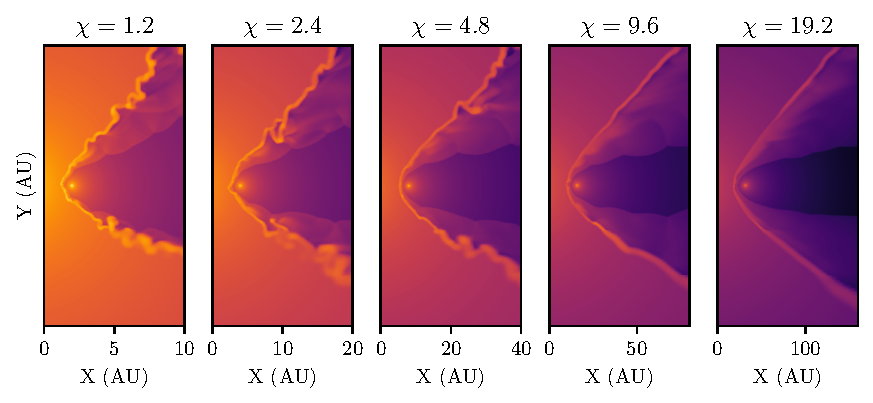
\includegraphics{assets/cwb-structure/ch1-chi-rho.pdf}
  \caption{A comparison of the influence of radiative cooling on the structure of a CWB system. A system with a momentum ratio of $\eta = 0.02$ is simulated with an increasing orbital separation, such that $\chi$ increases. As can be seen the WCR becomes adiabatic and smooth the more $\chi\rms{WR}$ increases.}
  \label{fig:chicomparison}
\end{figure}

\subsubsection{Dust cooling}
\label{sec:dustcooling-background}

\begin{figure}[h]
  \centering
  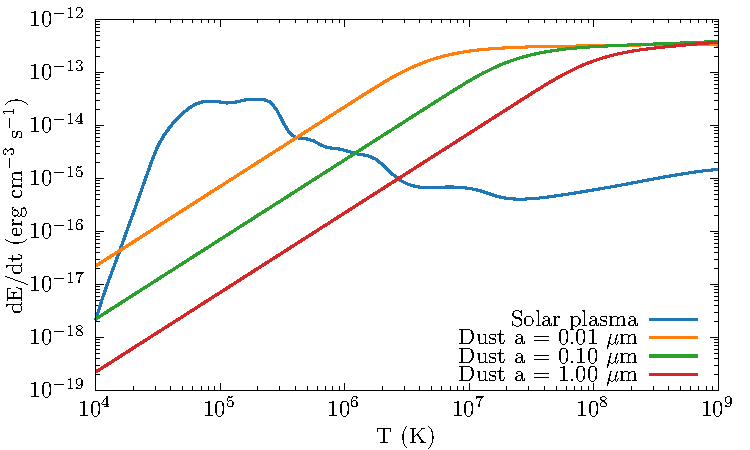
\includegraphics{assets/dust-plasma-cooling-comparison/cooling-comparison.pdf}
  \caption[Dust cooling vs. plasma cooling]{Comparison of plasma cooling to dust cooling with different grain sizes in a solar abundance gas, with a gas density of \SI{1e-20}{\gram\per\centi\metre\cubed} and a dust-to-gas mass ratio of 0.01.}
  \label{fig:dustplasmacomparison}
\end{figure}

Other radiative processes outside of gas/plasma cooling can influence the WCR.
Interstellar dust can have a significant impact on cooling in dust producing CWB (WCd) systems.
Collisional excitation and adsorption of photons can stochastically heat dust grains.
This excess energy is then emitted in the form of infrared radiation \parencite{dwekCoolingSputteringInfrared1996}.
The radiative emittance of a dust grain can be approximated as a black body, and hence radiates in accordance with the Stefan-Boltzmann law:

\begin{equation}
  L = 4\pi r^2 \sigma T^4 , 
\end{equation}

\noindent
where $L$ is the grain luminance, $r$ is the grain radius, $\sigma$ is the Stefan-Boltzmann constant\footnote{\SI{5.670e-5}{erg.cm^{-2}.s^{-1}.K^{-4}}.} and $T$ is the grain temperature.
At sufficiently high gas densities this radiative process can become the dominant cooling method in the ISM \parencite{wolfireNeutralAtomicPhases1995}.
In addition to this continuum emission, emission lines can also occur if characteristic vibrational modes in a grain lattice are excited, such as the silicate grain stretching and bending vibrational modes at \SI{9.7}{\micro\metre} and \SI{18.5}{\micro\metre} \parencite[212]{whittetDustGalacticEnvironment2002}, as well as the \SI{2175}{\angstrom} feature associated with PAHs \parencite{draineInterstellarDustGrains2003}.
% Dust cooling? Might need to move CWB dust formation up
The presence of dust within the immediate post-shock environment significantly increases the cooling rate, but is dependent on more than just the number density of the gas and the temperature.
In order to parametrise this, an energy loss rate, as formulated in Eq. \ref{eq:energylossrate} but for a volume of dust, $\mathcal{L}\rms{d}$ is used:

\begin{equation}
  \mathcal{L}\rms{d} (a,T) = n\rms{d} n\rms{g} \Lambda\rms{d} (a,T)
\end{equation}

\noindent
where $n\rms{d}$ is the number density of dust grains in the region and $a$ is the grain radius.
Fig. \ref{fig:dustplasmacomparison} compares $\mathcal{L}\rms{g}$ for a solar abundance plasma and $\mathcal{L}\rms{d}$ for dust within this plasma at varying grain sizes.
% As we can see, small grain sizes, with the same dust-to-gas mass ratio, dust cooling dominates at high temperatures, before reaching a peak emission rate.
At high temperatures we see that dust cooling is orders of magnitude more efficient.

Work by \textcite{dwek_infrared_1981} is used throughout this thesis to determine the rate of heating.
Collisional heating of dust grains from either gas, plasma or free electrons is assumed to be the primary mechanism of heating, with dust grains radiating this collisional energy on timescales much shorter than the collisional timescale.
It is found that the grain heating rate, $H$, can be calculated with the formulae:

\begin{equation}
  \label{eq:grainheatingrate}
  \begin{split}
    H & = \left(\frac{32}{\pi m}\right)^{1/2} n\pi a^2 (k_B T)^{3/2} h(a,T) \\
    & = \num{1.26e-19} \frac{n}{A^{1/2}} a^2 (\si{\micro\metre}) T^{3/2} h(a,T) \, \si{\erg\per\second}
  \end{split}
\end{equation}

\noindent
where $m$ is the grain mass, $a$ is the grain radius, $A$ is the mass of the incident gas particle in \si{\atomicmassunit}, and $n$ is the gas number density.
$h(a,T)$ is the effective grain ``heating factor'', or the fraction of the energy deposited into the grain through collision.
The calculation of $h(a,T)$ was found to be difficult when simulating CWB systems.
This is discussed in more detail in Section \ref{sec:dustcoolingmodel}.
Radiative heating is not calculated, as it is assumed that the dust grains are well shielded in the WCR from the UV emission of the parent stars.
The contribution of heating due to each ion species and electron is individually calculated, and combined to find the total grain heating rate:

\begin{equation}
  H = H\rms{el} + \sum_i H_i , 
\end{equation}

\noindent
where $H_i$ is the grain heating due to collisions from an element, $i$.
Whilst collision from atoms and ions is a somewhat important factor in grain heating, we find that the primary contribution of grain heating is due to electron-grain collisions.
As can be seen in \ref{fig:collisionalheatingcomparison}, heating due to electrons peaks between $10^5$ and $10^6 \, \si{K}$, with a ratio of contributions from electrons to ions of $\sim 100 : 1$.
This is partially due to the increased electron number density, as the plasma can be multiply or completely ionised at higher temperatures.
This is significant in the case of high-metallicity winds.
However, above $10^6\,\si{K}$ the electrons become less efficient at the heating of grains, resulting in a decreased influence in the overall grain cooling rate.
The heating factor decreases as the electrons become too energetic, and can pass through the grain without significant energy transfer.
This impact is especially important on small grains, as there is less material for the electrons to pass through.

\begin{figure}[h]
  \centering
  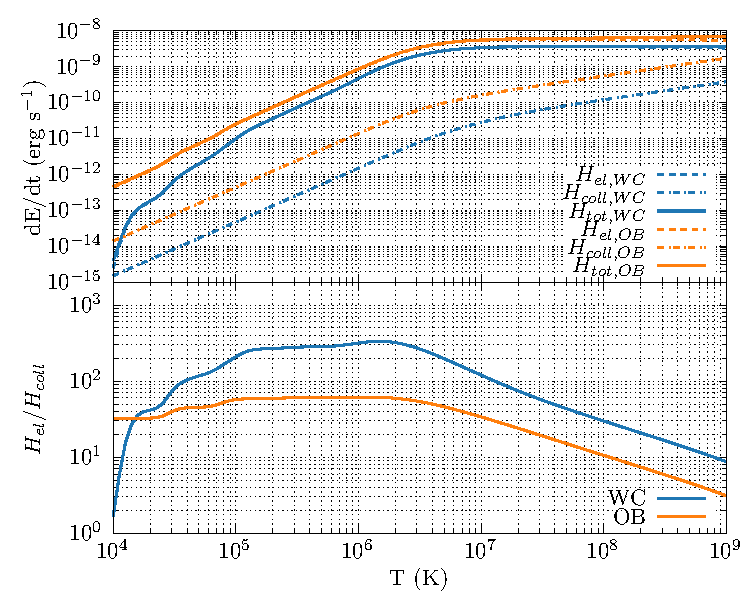
\includegraphics{assets/dust-electron-contribution/coll-el-comp.pdf}
  \caption[$H_{el}$ and $H_{coll}$ comparison]{Comparison of grain heating rate due to ion collisional excitation, $H_{coll}$, and electron excitation, $H_{el}$. The dust grain has a grain radius of \SI{5e-3}{\micro\metre} and is in a gas with a density of $10^{-20}$ \si{\gram\per\centi\metre\cubed} with solar and WC abundances.}
  \label{fig:collisionalheatingcomparison}
\end{figure}

\subsection{Dust formation in CWB systems}
\label{sec:cwbdust}

%Intro to dust formation in said systems
Despite the extremely violent conditions thus far described in CWB systems, these systems appear to be extremely prolific producers of interstellar dust.
Whilst single WC stars can produce small amounts of dust in the form of amorphous carbon grains (though this could be observed to be extremely rare, pending the results of \textcite{medinaAreAllWCd2021}), binary systems have been observed to convert more than 10\% of their wind masses from ionised carbon into amorphous carbon dust grains\footnote{In extreme cases.}.
This can result in a dust production rate in excess of $10^{-6} \, \si{\solarmass\per\year}$, more than a typical AGB star.
The dust production rate ranges from $10^{-10}$ to $10^{-6}\, \si{\solarmass\per\year}$ \parencite{lauRevisitingImpactDust2020}.
Research by \textcite{zubkoPhysicalModelDust1998a} details dust growth around these regions.
Grains were found to rapidly form from impinging carbon ions, up to grain sizes of approximately $100-200 \, \si{\angstrom}$.
This dust forming behaviour has only been observed in cooler WC stars (predominantly WC9, with some WC7-8 examples).
WN and WO systems have not been observed producing dust, this is most likely due to amorphous grains being significantly more chemically stable and resilient to effects such as sublimation and photoevaporation than water ice or silicate grains \parencite{salpeter_formation_1977,draineDestructionMechanismsInterstellar1979}.
Dust formation is also observed to form within the WCR, which can form quite beautiful pinwheel-shaped patterns, as dust streams away from the stars in the post-shock outflow.

\begin{table}[h]
  \centering
  \begin{tabular}{lllllll}
    \hline
    & \multicolumn{2}{l}{Persistent} & \multicolumn{2}{l}{Variable} & \multicolumn{2}{l}{Episodic} \\ \cline{2-7} 
    & Total & Example & Total & Example & Total & Example \\
    \hline
    WC4 & 1 & WR19 & 0 & --- & 0 & --- \\
    WC5 & 0 & --- & 0 & --- & 1 & WR47C \\
    WC6 & 1 & WR124-10 & 0 & --- & 0 & --- \\
    WC7 & 3 & WR102-22 & 0 & --- & 4 & WR140 \\
    WC8 & 6 & WR13 & 1 & WR48a & 3 & WR122-14 \\
    WC9 & 45 & WR104 & 6 & WR98a & 1 & WR75-11 \\ \hline
    Total & 56 &  & 7 &  & 9 &  \\ \hline
  \end{tabular}
  \caption[Number of confirmed WCd systems]{Number of confirmed WCd systems with known spectral type and dust formation type from the Galactic Wolf-Rayet Catalogue \parencite{rossloweSpatialDistributionGalactic2015}, systems with uncertain spectral types not included, while systems labelled ``d'' are included within the ``persistent'' category for their associated spectral type.}
  \label{tab:wc-summated-list}
\end{table}

% Rarity
Whilst beautiful, Wolf-Rayet systems are elusively rare.
The \footlink{Galactic Wolf-Rayet Catalogue}{http://pacrowther.staff.shef.ac.uk/WRcat} \parencite{rossloweSpatialDistributionGalactic2015} has a collection of 667\footnote{At time of time of writing, with the last update being August 2020.} known galactic WR stars.
106 of such stars are contained within a binary system, with 41 such binaries containing WC stars.
\textcite{rossloweSpatialDistributionGalactic2015} notes that there are a total of 42 confirmed WCd systems, approximately 35\% of all WC systems, though this value is somewhat out of date and includes single star systems.
A more up-to-date estimate performed for this thesis using the updated dataset estimates a total of 80 WCd systems, of which 72 have well-determined spectral subtypes (Table \ref{tab:wc-summated-list} \& Fig. \ref{fig:wrmap}).
% Impact of systems 
\textcite{rossloweSpatialDistributionGalactic2015} goes on to estimate that out of an estimated total of 1900 galactic WR stars, approximately 300 of these stars are predicted to be dusty WC stars.
Whilst this is a far cry from the number of galactic AGB stars, which outnumber WCd stars by approximately 3 orders of magnitude \parencite{ishiharaGalacticDistributionsCarbon2011}, these systems can still significantly impact the surrounding interstellar medium -- with strong stellar feedback propagating large quantities of dust into the surrounding medium.

\begin{figure}[h]
  \centering
  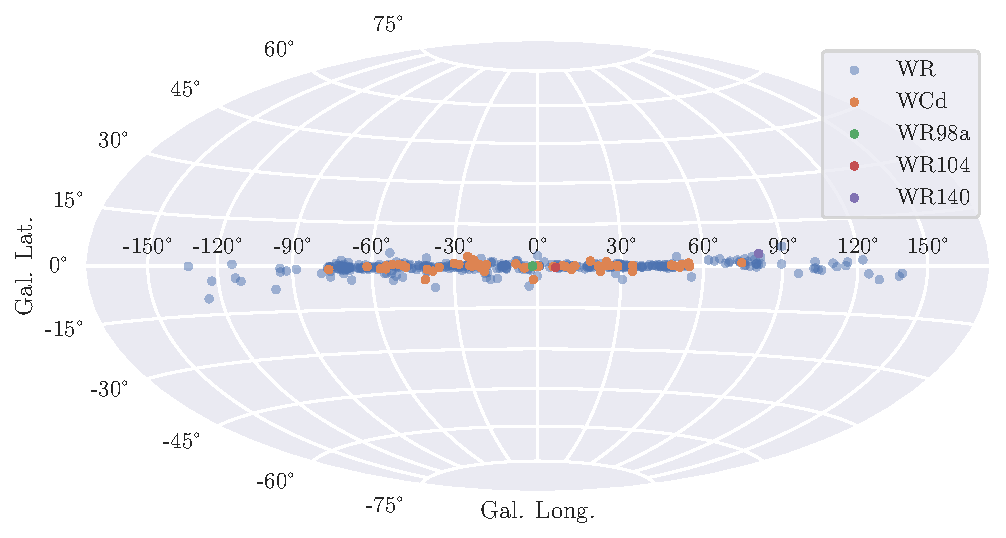
\includegraphics[width=\linewidth]{assets/galactic.pdf}
  \caption[Map of WR stars on the galactic plane]{Map of WR stars on the galactic plane. WCd systems have been highlighted, as well as the simulated systems in this thesis, WR98a, WR104 and WR140.}
  \label{fig:wrmap}
\end{figure}

% Number of WCd systems, reasoning for only certain subtypes being dust forming
Table \ref{tab:wc-summated-list} contains an excerpt of the observed WCd systems with clearly defined spectral subtypes.
Most dust producing stars are either WC8 or WC9 subtypes, which are markedly cooler and less luminous than their WC4 counterparts.
This reduced luminosity is potentially the driving factor for dust formation in the system.
As WC8-9 systems have slower, cooler winds \parencite{niedzielskiKinematicalStructureWolfRayet2002}, they are more strongly influenced by post-shock cooling, allowing for greater dust formation within the WCR.
A small number of these systems have somewhat variable or episodic dust production cycles, such as WR98a and WR140, which are the two systems being simulated in this thesis.
Furthermore, the bulk of WCd systems do appear to be in binary systems with a close periastron passage.
In fact, the orbit appears to be a driving force behind how dust is produced in these systems, as we will later discuss.

%Theories as to why
A good starting point to understanding dust formation is to understand how the WCR can mitigate the mechanisms resulting in dust destruction, whilst aiding the processes involved in dust formation.
As previously discussed, dust can be destroyed through high-velocity collisions with grains, as well as evaporation through heating or ionising radiation.
These processes are mitigated through the cooling, as well as through the large amount of UV extinction due to the high density of the WCR.
Meanwhile, the dust production rate increases within high density regions, as collisions between dust grains and gas occur at a much higher rate.
The same can be said with dust grains, allowing for fast growth from gas and impinging ion accretion, and grain-grain collision as the number density of dust grains begins to increase.
The accumulation of these effects results in a very fast initial growth rate, which tapers off as the post-shock region diffuses and expands.

% Role of instabilities
The presence of instabilities driven by cooling and other factors leads to pockets of high density post-shock material.
This can lead to ``clumps'' of highly dust-enriched post-shock stellar wind.
These clumps would have additional protection from UV photons, and would also be cool enough for dust to form.
Thus, the driving hypothesis for this theory is that these are regions where the bulk of dust formation would occur.
% How to make lots of dust + reminder of aims of project.
Therefore, in order to achieve a high rate of dust formation, a dense, highly radiative post-shock WCR must be formed.
As cooling in the post-shock region is dependent on separation distance, wind velocity and mass loss rate, these parameters should first be explored, with the knowledge gleaned used to direct an analysis of observed systems such as WR140.

%Observational data Link to Crowther papers in particular, dust formations only around WC
% Discuss role of eccentricity
Eccentricity is also theorised to play an important factor in the production of dust.
We observe that highly eccentric systems can vary their dust production rates significantly.
Fig. \ref{fig:periodicmags} shows the periodic change in mid-IR emission that can be explained as dust emission from small amorphous carbon grains, in the case of systems such as WR140 or WR125 dust production is periodically reduced to the point where associated emissions can drop by several magnitudes.
This relation is clearly periodic, with a peak in dust production coinciding with the periastron passage of these systems.
This implies that dust production is dependent on orbital separation, which will influence the degree of cooling occurring within the WCR, it could potentially also alter the wind velocity on collision, which will also influence dust production in the same manner.
% Metastudy
Further analysis of available dust producing CWB systems suggests that many WCd systems with circular orbits produce dust either persistently or with a degree of variability, while eccentric WCd systems solely produce dust episodically \parencite{crowther_dust_2003,williamsVariableDustEmission2019}.

\begin{figure}[h]
  \centering
  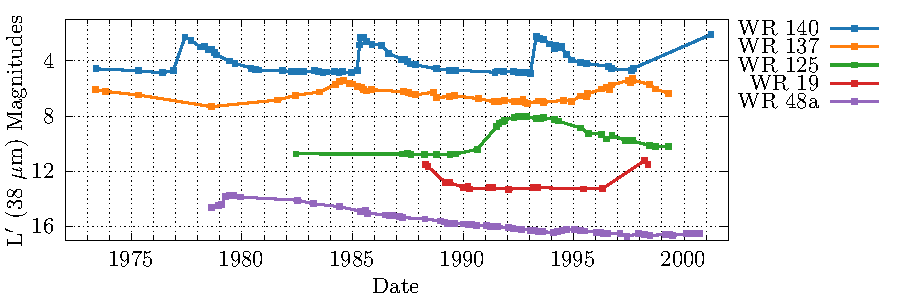
\includegraphics[]{assets/magnitudes/magnitudes.pdf}
  \caption[L$^\prime$ photometry of episodic dust making stars]{L$^\prime$ photometry for episodic dust making stars, data derived from \textcite{crowther_dust_2003}, and provided by PM Williams in private correspondence. WR140 and WR137 in particular have extremely predictable dust forming events which correspond to periastron passage in both systems.}
  \label{fig:periodicmags}
\end{figure}


\subsection{Important WCd systems}

The principle systems that are being simulated in this thesis are the variable dust forming system WR98a, and the episodic dust forming system WR140.
The archetypal continuous dust forming system WR104 was also considered for simulation, but had to be cut due to time constraints.
This system will also be discussed to provide a point of comparison between the two systems.

\begin{table}[h]
  \centering
  \begin{tabular}{llllllll}
  \hline
  System & $\dot{\text M}_{\text{WR}}$ & $\dot{\text M}_{\text{OB}}$ & $v_{\text{WR}}^\infty$ & $v_{\text{OB}}^\infty$ & $\eta$ & $\chi_\text{WR,min}$ & $\dot{\text M}_\text{D}$ \\
   & (\si{\solarmass\per\year}) & (\si{\solarmass\per\year}) & (\si{\km\per\second}) & (\si{\km\per\second}) & & & (\si{\solarmass\per\year}) \\ \hline
  WR98a & \num{5.0e-6} & \num{5.0e-8} & 900  & 2000 & 0.0222 & 0.7970 & $\left(6.10^{+1.77}_{-1.38}\right) \times 10^{-7}$ \\ 
  WR104 & \num{3.0e-5} & \num{6.0e-8} & 1220 & 2000 & 0.0033 & 0.2430 & $\left(4.39^{+1.27}_{-0.97}\right) \times 10^{-6}$ \\
  WR140 & \num{5.6e-5} & \num{1.6e-6} & 2895 & 3200 & 0.0314 & 2.6866 & $\left(8.11^{+4.83}_{-4.15}\right) \times 10^{-10}$ \\ \hline
  \end{tabular}
  \caption[Wind properties of systems considered for simulation]{Wind properties of systems considered for simulation in this thesis.}
  \label{tab:systems-wind-properties}
\end{table}

\begin{table}[h]
  \centering
  \begin{tabular}{lllllllll}
  \hline
  System & Classification & Period & Eccentricity & Inclination & $M_{\text{WR}}$ & $M_{\text{OB}}$ & Periastron & Apastron \\
   & & (d) & ($e$) & ($i$) & (\si{\solarmass}) & (\si{\solarmass}) & (AU) & (AU) \\ \hline
  WR98a & WC8-9+OB & 556 & $\sim 0$ & $35\pm6^\circ$ &10.0 & 18.0 & 4.06 & 4.06 \\
  WR104 & WC9d+B0.5V & 245 & 0.0600 & $\lesssim 16^\circ$ & 10.0 & 20.0 & 2.20 & 2.48 \\
  WR140 & WC7+O5 & 2869 & 0.8993 & $119.1\pm0.9^\circ$ & 10.31 & 29.27 & 1.53 & 26.9 \\ \hline
  \end{tabular}
  \caption[Orbital properties of systems considered for simulation]{Orbital properties of systems considered for simulation in this thesis.}
  \label{tab:systems-orbital-properties}
\end{table}

\subsubsection{WR98a}

\begin{figure}[h]
  \centering
  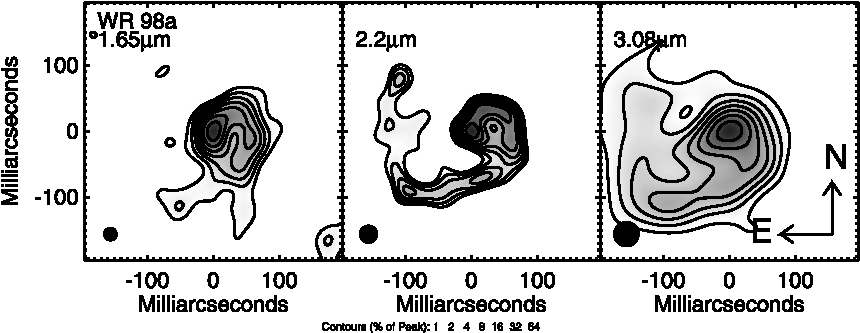
\includegraphics{assets/systems/wr98a-monnier2007.pdf}
  \caption[\textit{Multiwavelength image of WR98a \parencite{monnierKeckAperturemaskingExperiment2007}}]{Multiwavelength aperture synthesis images of WR98a taken on June \nth{24} 2000, at 1.65, 2.2, and \SI{3.08}{\micro\metre}. Plot sourced from \textcite{monnierKeckAperturemaskingExperiment2007}, the significant IR excess is a clear sign of ongoing dust production. The system also has a pronounced pinwheel structure most prominent at \SI{2.2}{\micro\metre}.}
  \label{fig:wr98aimage}
\end{figure}

% Historical observation 

WR98a (Fig. \ref{fig:wr98aimage}) was first found to be a WCd system by \textcite{monnierPinwheelNebulaWR1999}, and for a number of reasons was found to be an ideal candidate for simulation.
% Ease of simulation, good starting point
WR98a was chosen for simulation primarily due to its moderate rate of dust formation, and comparatively docile winds.
With a slow WC wind velocity of \SI{900}{\kilo\metre\per\second} and a WC mass loss rate of \SI{5e-6}{\solarmass\per\year}, it has an overall WC wind momentum far lower than the other candidate systems.
Because of this, the system has far lower dust production rates, and also exhibits some dust variability \parencite{lauRevisitingImpactDust2020}.
Due to these factors the system is markedly easier to simulate, and thus provided a good starting point for our work as we refined the model and implemented features into the hydrodynamical system.
A comparatively wide orbit reduces the number of cells required to simulate the system, as the WCR is easily resolved from the OB star, simplifying the simulation of the system further.
Finally, WR98a has previously been simulated using a multi-fluid dust model in \textcite{hendrix_pinwheels_2016}, this allows us to provide a point of comparison between our work and already published work.
This is especially useful as there are only a handful of papers that cover dust models in CWB systems.
% Parameter space exploration
Because of this relative ease of simulation and relatively slow wind velocity for both stars in the system, WR98a was chosen to be the baseline system for the research conducted in chapter \ref{chap:parameterspace}.

\subsubsection{WR140}

% Historical observation
WR140 is significant in that it is the first system observed with episodic WCd properties.
\textcite{williamsCondensationShellHD1978} noted a rapid brightening in the infrared, suggesting the formation of a new shell of dust around the system.
WR140 has been observed many times over the years, with spectroscopic data dating back to 1972, and is perhaps the most well-observed episodic WCd system.
% Eccentric orbit, variable dust formation
With its eccentricity of $e=0.8993$, the separation between the stars -- and therefore $\chi$ -- vary by a factor of 17.6 from apastron to periastron.
Therefore it an ideal system to verify that our dust model can naturally handle episodic dust forming systems, as well as to determine which parameters affect an episodic system.

% Difficulty of simulation
As it is a highly eccentric system with a particularly long period orbit, a number of difficulties present themselves.
Firstly, the system has a much longer orbital period than the other systems being considered, as such, a complete orbit would take a long time to simulate as well.
Secondly, this requires a corresponding increase in resolution, as the WCR needs to be sufficiently resolved at periastron.
Whilst refinement methods such as Adaptive Mesh Refinement (AMR) would alleviate these issues somewhat, we found that the current version of the \athena{} hydrodynamical code lacked stability with passive scalars in AMR.
This issue was deeply embedded in \athena{}, and as such could not be fixed by the end of this PhD.
% Snippet
Instead, it was decided to only simulate the system as it undergoes closest approach, from $\phi = 0.95$ to $\phi = 1.10$. 

\subsubsection{WR104}

\begin{figure}[h]
  \centering
  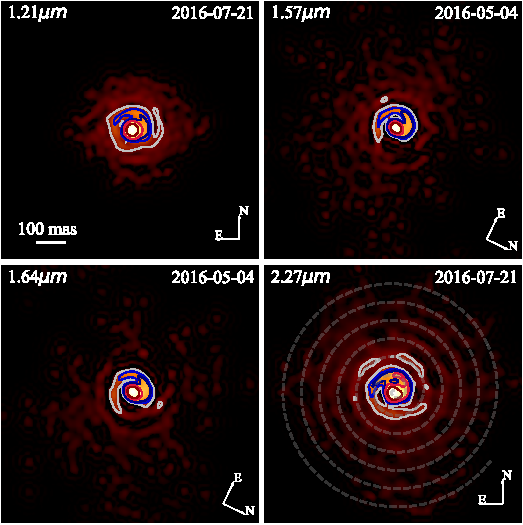
\includegraphics[]{assets/systems/soulain-2018-wr104.pdf}
  \caption[\textit{Spiral structure of WR104 \parencite{soulainSPHEREViewWolfRayet2018}}]{Deconvolution of J, H, K, and \SI{2.27}{\micro\metre} bands of WR104 sourced from \textcite{soulainSPHEREViewWolfRayet2018}. The spiral pattern and first revolution is visible in all images, in particular at \SI{2.27}{\micro\metre}.}
  \label{fig:soulain-wr104}
\end{figure}

% Physical properties
\noindent
WR104 (Fig. \ref{fig:soulain-wr104}) is an archetypal example of a continuous WCd system.
It is a comparatively tight binary with a semi-major axis of \SI{2.34}{\au} and a period of $\sim 241$ days.
The system also has a relatively circular orbit, with an eccentricity of $e = 0.06$ \parencite{lamberts_colliding_2012}.
WR104 consists of a WC9 star with a B0.5V partner \parencite{williamsSpectroscopyWC9WolfRayet2000}; this combination of a WC star and a comparatively weak B partner results in a severely imbalanced wind.
We estimate a wind momentum ratio of $0.003$, an order of magnitude lower than WR98a.
This imbalanced wind -- combined with the tight orbit -- results in an extremely IR bright WCR that is constantly churning out dust.
% Mass loss rate
Using radiative transfer models, \textcite{harriesThreedimensionalDustRadiativetransfer2004} calculated a dust production rate of \SI{8(1)e-7}{\solarmass\per\year}, corresponding to 2\% of the total mass loss rate of the system.
A more advanced model by \textcite{lauRevisitingImpactDust2020}, which is used to assess the dust formation rates of systems in this thesis, calculated the dust formation rate to be $\left(4.39^{+1.27}_{-0.97}\right) \times 10^{-6}\, \si{\solarmass\per\year}$.
This is one of the most prolific dust forming systems found by \textcite{lauRevealingEfficientDust2021}, and as such is an ideal example of a continuous dust forming system.
There are a number of reasons for this prodigious dust formation rate.
As the system's orbit is comparatively close and circular with a very dense primary wind, the wind is expected to be highly radiative throughout the entire orbital period, this suggests a cool post-shock WCR, which continuously produces dust.

% Why is it archetypal 
The system is relatively close, at a distance of \SI{2.5}{\kilo\parsec}, and is almost face-on relative to earth, meaning that the pinwheel structure is clearly observed (\cite{soulainSPHEREViewWolfRayet2018}; Fig. \ref{fig:soulain-wr104}).
Due to the system parameters, well defined dusty pinwheel structure, and prior observations and simulations of the system, it was found to be an ideal candidate for simulation.

% Why it wasn't assessed, difficulty of simulation, needed AMR
Despite being a very strong candidate for simulation, however, attempting to simulate the system proved to be exceptionally difficult.
% Many level simulation required for large-scale observation
The very close orbit of the system would mandate a very high simulation resolution, increasing the amount of processing time required to finish the simulation.
Only simulating a small region would prevent the pinwheel from being formed and observed, which we would have ideally wanted to include.
% Instability required running at very low Courant number
In addition the strong radiative cooling resulted in a test simulation being very unstable unless the Courant number was exceedingly small.
As timestep is governed by the Courant number, this would significantly increase the time needed to simulate the system.
With a limited amount of compute resources as well as a limited amount of time, this stretched the feasibility of simulating this system.
% Physical effects, gayley
As the wind from the primary star is significantly stronger than its partners, WR104 has a much lower momentum ratio than the other systems being considered, and the WCR is situated much closer to the secondary star.
At closest approach, $r_\text{OB} \approx \SI{60}{\solarradius}$, which would require WR104 to be simulated at a much higher resolution, in turn further increasing computational requirements.
Physical effects, such as radiative inhibition and sudden braking may also significantly alter the wind velocity and post-shock environment, reducing the pre-shock primary wind velocity \parencite{gayley_sudden_1997}.
The pre-shock secondary wind velocity would also be influenced, due to insufficient acceleration from line driving before the winds collide.
As radiative line driving is not simulated these effects cannot be taken into account, and would have resulted in an inaccurate simulation of the system.
Sudden braking in highly wind-imbalanced systems is discussed more substantially in section \ref{sec:simassumptions}.

% Why it was discarded
With limited time remaining in the project, as well as the above factors, simulation work on WR104 was abandoned in favour of a parameter space search of a system with baseline properties similar to WR98a, as well as a limited simulation of WR140.

Simulating this system however, is a particularly enticing avenue of future research.

\subsection{WR+WR systems}

Recently, two candidates of a theorised subset of CWB have been discovered: WR+WR systems.
These double WR systems have a secondary stellar wind around 3 orders of magnitude denser than a WR+OB system.
This would of course results in truly titanic wind collisions.
These candidates are the recently discovered WR70-16 \parencite{callinghamAnisotropicWindsWolf2019}, and the previously discovered WR48a system \parencite{danksInfraredSpectroscopyInfrared1983}, which exhibits the spectroscopic lines of both a WC and WN system \parencite{williamsVariableDustEmission2019}.
These systems are predicted to be comparatively rare, even among CWB systems.
This is due to the unlikelihood that both stars in the system would be in their Wolf-Rayet phase at the same time.
Despite these systems having an enormous combined mass-loss rate, initial estimates of the dust production rates of both systems indicate that their dust conversion efficiencies are comparatively low compared to less energetic systems, and overall quite mundane dust production rates in general.
Whether this suppressed dust production rate is a common phenomena among WR+WR systems remains to be seen, as more systems would need to be discovered in order to determine this.
Extragalactic WR+WR binaries have also been detected in the Magellanic clouds, though these are typically WN+WN pairs \parencite{shenarWolfRayetBinaries2019}.

\subsubsection{WR70-16 (``Apep'') -- a recently discovered WR+WR system}
\label{sec:bg-apep}

\begin{figure}[h]
  \centering
  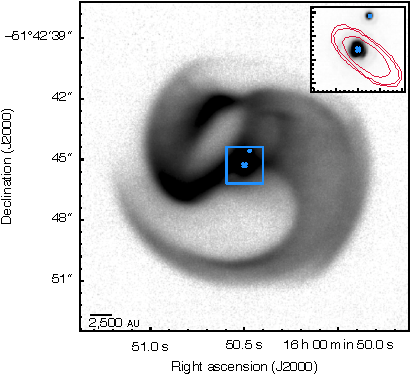
\includegraphics[]{assets/systems/apep-callingham-2019.pdf}
  \caption[\textit{VLT image of Apep \parencite{callinghamAnisotropicWindsWolf2019}}]{A VLT image of Apep \parencite{callinghamAnisotropicWindsWolf2019}, a recently discovered WR+WR system with a WN primary and WC secondary star. This class of system presents an interesting avenue of future research; though these systems are extremely rare.}
  \label{fig:apep-callingham}
\end{figure}

A potential avenue of research for this field is the simulation of WR+WR systems such as the recently discovered WR70-16 (Fig. \ref{fig:apep-callingham}) system (hereafter referred to as ``Apep'').
This system was discovered due to the significant difference between the spectroscopically derived wind velocity of \SI{3400(200)}{\kilo\metre\per\second} and the observed expansion speed of \SI{570(70)}{\kilo\metre\per\second} \parencite{callinghamAnisotropicWindsWolf2019}.
This inhibited wind velocity, far below any categorised WR wind velocity, suggests that much of the wind undergoes collision with the wind of a binary partner.
The extremely luminous non-thermal and infrared emission, suggested two extremely high mass loss rate stars within the system, as well as evidence for a third, distant partner in a loose triple system \parencite{callinghamTwoWolfRayet2020}.
Spectroscopic analysis suggested that the central component of the Apep system consists of a nitrogen sequence WN4-6b and a carbon sequence WC8 star, with the more massive and luminous WN4-6b star kinematically dominating the system.
This discovery is very significant as it was the first galactic WR+WR system discovered -- and is only one of two galactic WR+WR systems. Other systems have been identified, but are extragalactic in nature.

Further work by \textcite{hanExtremeCollidingwindSystem2020} has estimated the orbital parameters of Apep, finding that it is a highly eccentric system with a period of \SI{125(20)}{\year} and an eccentricity of \num{0.7(0.1)}, inclined at $\pm \ang{30} \pm \ang{5}$ towards Earth.
An initial estimate of the dust formation rate was made, finding a dust production rate of $\sim \SI{5e-7}{\solarmass\per\year}$, while observation of the surrounding dust shell suggests that it is a periodic dust forming system, which is sensible considering the systems high eccentricity.
The opening angle of the WCR was found to be very wide, at $\ang{125}\pm\ang{10}$, further suggesting the presence of two very high mass loss rate objects within the system due to a balanced wind momenta.
Additional calculations by \textcite{marcoteAUscaleRadioImaging2021} estimated the systems wind momentum ratio to be $0.44\pm 0.08$, again in line with the WR+WR hypothesis. 
Finally, the pre-print by \textcite{delpalacioNonthermalEmissionCollidingwind2021} finds a mass loss rate of \SI{4e-5}{\solarmass\per\year} for the WN star and \SI{2.9e-5}{\solarmass\per\year} for the WC star, which all but confirms the presence of a WR+WR binary at the heart of the Apep system.

With an estimated combined mass loss rate of \SI{6.9e-5}{\solarmass\per\year} we estimate that the system has a dust conversion efficiency of 0.7\%.
Whilst this system is therefore not a prodigious producer of dust, this is most likely due to the extremely high wind terminal velocity and high separation distance, which would suggest a fairly smooth and adiabatic post-shock region. 
We can estimate the cooling parameter of the system to be $\sim 80$, based on the angular separation from \textcite{hanExtremeCollidingwindSystem2020}, confirming that at present, the winds are adiabatic.
It is most likely the case that the system is highly elliptic, and is currently dormant in a similar manner to WR140 is for most of its orbit.
In order to estimate the closest approach of the system, and therefore the minimum cooling parameter an accurate measure of the stellar mass of both objects would need to be made.
There is insufficient data for this at the time of writing.

\subsubsection{WR48a -- revisiting a WR+WR candidate}
\label{sec:bg-wr48a}

WR48a is a system that was previously considered to be a CWB system with a WR primary star and an unknown secondary star \parencite{zhekovMultiwavelengthViewDusty2014}.
Recently, however, it has been reclassified to a WR+WR system, with a dust forming WC8 and a WN8 partner \parencite{williamsVariableDustEmission2019,zhekovChandraRevisitsWR2022}.
This change in classification is contemporaneous with the discovery and classification of Apep, though there is a distinct lack of recent observations of this system compared to the newer, more exciting WR+WR candidate.
\textcite{lauRevisitingImpactDust2020} calculated a dust formation rate for WR48a of $\left(8.46^{+3.48}_{-4.38}\right) \times 10^{-8} \, \si{\solarmass\per\year}$ with a dust conversion efficiency of $0.12\%$, markedly less than other systems with much less available material.
A future avenue of research would be to simulate these systems to understand why the dust formation rate is comparatively low, despite the readily available stellar material.
The main difficulty of simulating these systems is the lack of orbital parameters and accurate mass loss rates.
As WR48a has insufficient data and Apep has only been recently discovered, there are currently too many unknown factors in order to build an adequate simulacrum of the systems\footnote{A lack of accurate orbital parameters is a significant issue in devising simulations for more conventional WR+OB systems}.
Another difficulty is the large degree of orbital separation, high eccentricity and long orbital timescales required to simulate these systems.
The current limitations of the hydrodynamical code being used in this project render it difficult to simulate entire orbital passes of highly elliptical systems with long periods.
If these issues are resolved in later versions of the hydro code however, this would present an interesting avenue of future research.
